\documentclass[slidestop,aspectratio=169]{beamer}
\usetheme{Pittsburgh}
\usepackage{listings}
\usepackage[utf8x]{inputenc}
\usepackage{etex}
\usepackage[setrelation]{math}
\usepackage[modernsign,substopindex,shortmquant,mquantifiertype,
mconnectiveformal,postfixflatinterpret,bracketmodalinterpret,
setfixinterpret,modifopindex,seqinfers,seqoptional,footnotecalculus,abbrseqcontext,shortterms,nosigmaterms,novarterms]{logic}
\usepackage[pretest,nocommandblocks]{progreg}
\usepackage[bracketinterpret,postfixinterpret,bracketmodalinterpret,simplenames]{dL}
\usepackage{tabularx,xcolor,colortbl}
\usepackage{subcaption}
\usepackage{booktabs}
\usepackage{todonotes}
\usepackage{wrapfig}
\usepackage{stmaryrd}
\usepackage{proof}
\usepackage{prettyref}
\usepackage{tikz}
\usepackage{pgfplots}
\usepackage{slidetool}
\usepackage[absolute,overlay]{textpos}
\usepackage{marvosym}
\let\Cross\undefined
\usepackage{bbding}
\usenavigationsymbolstemplate{}
\pgfplotsset{width=8cm,compat=1.9}
 \usetikzlibrary{arrows}
 \usetikzlibrary{calc}
 \usetikzlibrary{fit}
 \usetikzlibrary{positioning,shadows}
 \usetikzlibrary{automata}
 \usetikzlibrary{shapes,arrows}
 \usetikzlibrary{decorations.text}
 \usetikzlibrary{decorations.markings}
 \usetikzlibrary{trees,snakes}
\usetikzlibrary{pgfplots.dateplot}
\usepackage{relsize}
\tikzset{fontscale/.style = {font=\relsize{#1}}}
\usepackage{pgfplotstable}
\usepackage{filecontents}

\definecolor{vermillion}{rgb}{0.8,0.4,0}
\definecolor{myblue}{rgb}{0,0.45,0.7}
\definecolor{myyellow}{rgb}{0.85,0.8,0.17}


\newcommand{\rref}[2][]{\prettyref{#2}}

  \tikzstyle{noteline}=[shorten <=8pt]%
  \tikzstyle{notebox}+=[minimum height=1.1cm]%
\newrefformat{sec}{Section\,\ref{#1}}
\newrefformat{appendix}{Appendix\,\ref{#1}}
 \newrefformat{model}{Model\,\ref{#1}}
 \newrefformat{listing}{Listing\,\ref{#1}}
 \newrefformat{line}{line\,\ref{#1}}
 \newrefformat{def}{Definition\,\ref{#1}}
 \newrefformat{defn}{Definition\,\ref{#1}}
 \newrefformat{thm}{Theorem\,\ref{#1}}
 \newrefformat{ax}{\ref{#1}}
 \newrefformat{prop}{Proposition\,\ref{#1}}
 \newrefformat{lem}{Lemma\,\ref{#1}}
 \newrefformat{cor}{Corollary\,\ref{#1}}
 \newrefformat{ex}{Example\,\ref{#1}}
 \newrefformat{tab}{Table\,\ref{#1}}
 \newrefformat{fig}{Figure\,\ref{#1}}
 \newrefformat{eqn}{(\ref{#1})}
\renewcommand{\ivr}{\psi}
\providecommand{\tweak}[1]{#1}
\newcommand{\untweak}[1]{}
\newcommand{\ignore}[1]{}
\newcommand{\stdI}{\dLint[state=\nu]}%
\newcommand{\ws}{\nu}
\newcommand{\wt}{\omega}%
\newcommand{\I}{\iconcat[state=\ws]{\stdI}}%
\newcommand{\It}{\iconcat[state=\wt]{\stdI}}%
\definecolor{vgray}{rgb}{.35,.35,.35}
\renewcommand*{\irrulename}[1]{\text{\textcolor{vgray}{\upshape#1}}}
\usepackage{tikz}
\usepackage{stmaryrd}
\usetikzlibrary{arrows,matrix}
\newcommand{\isabelle}{Isabelle/HOL\xspace}
\newcommand{\allstate}{\mathcal{S}}
\newcommand{\tvm}{\oslash}
\newcommand{\tvt}{\oplus}
\newcommand{\tvf}{\ominus}
\newcommand{\term}{\mathbf{Term}\xspace}
\newcommand{\lequiv}{\leftrightarrow}
\newcommand{\state}{\mathbf{State}\xspace}
\newcommand{\prop}{\mathbf{Prop}\xspace}
\newcommand{\fml}{\mathbf{Fml}\xspace}
\newcommand{\dLi}{\ensuremath{\dL_{\iota}}\xspace}
\newcommand{\KeY}{KeY}
\newcommand{\tint}[2]{#2\lenvelope#1\renvelope}
\newcommand{\fint}[2]{#2\lenvelope#1\renvelope}
\newcommand{\pint}[1]{\lenvelope#1\renvelope}
\newcommand{\piint}[2]{#2\lenvelope#1\renvelope}
\newcommand{\meps}[2]{\iota{#1}\,{#2}}
\newcommand{\mepsIndef}[2]{\varepsilon{#1}\,{#2}}
\newcommand{\R}{\mathbb{R}}
\newcommand{\err}{\textsf{Err}\xspace}
\newcommand{\ffalse}{\textsf{false}\xspace}
\newcommand{\ftrue}{\textsf{true}\xspace}
\newcommand{\projGen}[2]{\ensuremath{\pi_{#1}}{#2}}
\newcommand{\projL}[1]{\projGen{1}{#1}}
\newcommand{\projR}[1]{\projGen{2}{#1}}
\newcommand{\inR}[1]{\textsf{in}{\ensuremath{\mathbb{R}}}(#1)}
\newcommand{\isT}[1]{\textsf{isT}(#1)}
\newcommand{\om}{\omega}
\newcommand{\tom}{\tilde{\omega}}
\newcommand{\tnu}{\tilde{\nu}}
\newcommand{\tmu}{\tilde{\mu}}
\newcommand{\denote}[1]{\mathsf{E}(#1)}
\newcommand{\llc}[3]{\mathsf{LLC}(#2(#1))}
\newcommand{\cont}[2]{\mathsf{Con}(#2(#1))}
\newcommand{\tder}[2]{\der{#2(#1)}}
\newcommand{\hasdiff}[1]{\mathsf{D}(#1)}
\newcommand{\vepsilon}{\xi}
\newcommand{\stepsto}{\allowbreak\mapsto\allowbreak}
\newcommand{\bebecomes}{\mathrel{::=}}
\newcommand{\alternative}{~|~}
\newcommand{\ProofPlex}{ProofPlex\xspace}
\newcommand{\ModelPlex}{ModelPlex\xspace}
\providecommand{\KeYmaeraX}{KeYmaera X\xspace}


% CdGL
\newcommand{\GL}{GL\xspace}
\newcommand{\CGL}{CGL\xspace}
\newcommand{\CdGL}{CdGL\xspace}
\newcommand{\dRL}{dRL\xspace}
\newcommand{\Isabelle}{Isabelle\xspace}
\newcommand{\CakeML}{CakeML\xspace}


\newcommand{\engineer}[1][1in]{
\includegraphics[width=#1]{img/rosie.png}}
\newcommand{\logician}[1][1in]{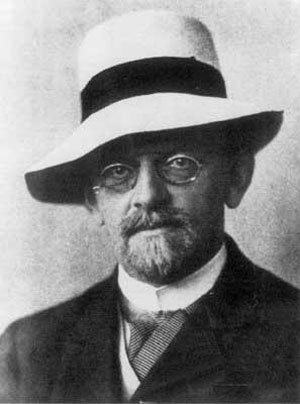
\includegraphics[width=#1]{img/hilbert.png}}
\newcommand{\logicuser}[1][1in]{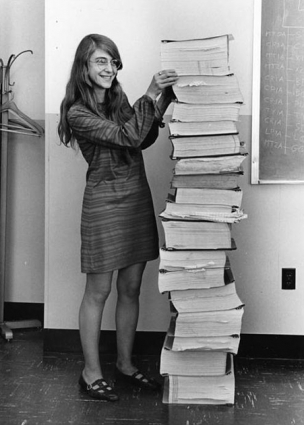
\includegraphics[width=#1]{img/hamilton.png}}


\newcommand{\speak}[2]{\small\begin{minipage}{1.3in}{#1}{#2}\end{minipage}}
\newcommand{\say}[1]{\speak{#1}{}}
\newcommand{\sayHappy}[1]{\speak{#1}{\Smiley}}
\newcommand{\saySad}[1]{\speak{#1}{\Frowny}}
\newcommand{\turn}{\textsc{Turn}}
\newcommand{\nim}{\textsc{Nim}}
\newcommand{\cake}{\textsc{CC}}


\newcommand{\rangevar}{\textsf{Range}}
\newcommand{\testvar}{\textsf{test}}
\newcommand{\elem}[2]{\textsf{Dec}[#1](#2)}
\newcommand{\spc}{\hspace{0.15in}}
\newcommand{\kwmod}{\textsf{mod}}
\newcommand{\emod}[2]{#1~\kwmod~#2}
\newcommand{\kwdiv}{\textsf{div}}
\newcommand{\ediv}[2]{#1~\kwdiv~#2}
\newcommand{\kwsig}{\Sigma}
\newcommand{\sig}[1]{\kwsig(#1)}
\newcommand{\interp}{I}
\newcommand{\valset}[1]{\mathfrak{V}(#1)}
\newcommand{\kwbool}{\m{\mathbb{B}}}
\newcommand{\kwint}{\m{\mathbb{Z}}}
\newcommand{\kwreal}{\m{\mathbb{R}}}
\newcommand{\kwintsig}{\Xi}
\newcommand{\intsig}[1]{\kwintsig(#1)}
\newcommand{\churchkleene}{\omega_{\text{CK}}}
\newcommand{\restL}[1]{#1_L}
\newcommand{\restR}[1]{#1_R}
\newcommand{\apL}[1]{#1_{\langle{0}\rangle}}
\newcommand{\apR}[1]{#1_{\langle{1}\rangle}}
\newcommand{\dpL}[1]{#1_{[0]}}
\newcommand{\dpR}[1]{#1_{[1]}}

\newcommand{\va}{a}
\newcommand{\vb}{b}
\newcommand{\vca}{\overline{a}}
\newcommand{\vcb}{\overline{b}}

\newcommand{\btt}{\texttt{tt}}
\newcommand{\bff}{\texttt{ff}}
\newcommand{\stt}{\top}
\newcommand{\sff}{\bot}
\newcommand{\demonactive}[2]{\textrm{aD}(#1,#2)}
\newcommand{\demondormant}[2]{\textrm{dD}(#1,#2)}
\newcommand{\sren}[3]{\urename[{#1}]{#2}{#3}}%{\subst[{#1}]{#2}{#3}}
\newcommand{\ssub}[3]{\subst[{#1}]{#2}{#3}}
\newcommand{\eren}[3]{\urename[{#1}]{#2}{#3}}%{\subst[{#1}]{#2}{#3}}
\newcommand{\earen}[2]{\urename[{#1}]{\boundvars{#2}}{\vec{y}}}%{\subst[{#1}]{\boundvars{#2}}{\vec{y}}}

\newcommand{\allcon}{\allregion}
\newcommand{\somesemi}[2]{\epsilon #1~|~#2}

\newcommand{\rzF}[2]{#1 \vdash #2}
\newcommand{\rzA}[3]{\langle{#2}\rangle(#1)=(#3)}
\newcommand{\rzD}[3]{[{#2}](#1)=(#3)}
\newcommand{\rzFst}[1]{#1_0}
\newcommand{\rzSnd}[1]{#1_1}
\newcommand{\rzThd}[1]{#1_2}
\newcommand{\rzFrt}[1]{#1_3}
\newcommand{\rzApp}[2]{#1\,#2}
\newcommand{\sa}{\omega}
\renewcommand{\sb}{\nu}
\newcommand{\Sc}{\mu}
\renewcommand{\aa}{a}
\newcommand{\ab}{b}
\newcommand{\ac}{c}
\newcommand{\da}{d}
\newcommand{\db}{D}
\newcommand{\dc}{\DJ}
\newcommand{\allRz}{\mathcal{R}\mathbf{z}}
\newcommand{\rzfor}[1]{#1\,\allRz}

\newcommand{\mto}{\rightharpoonup}
\newcommand{\esub}[3]{[{#3}/{#2}]{#1}}
\newcommand{\tsub}[3]{\subst[#1]{#2}{#3}}


%\newcommand{\rzF}[2]{#1 \vdash #2}
%\newcommand{\rzA}[3]{\langle{#2}\rangle(#1)=(#3)}
%\newcommand{\rzD}[3]{[{#2}](#1)=(#3)}
\newcommand{\rzNil}{\epsilon}
\newcommand{\rzCons}[2]{(#1,#2)}
\newcommand{\rzBLam}[2]{\lambda #1:\allstate.~#2}
\newcommand{\rzHOLam}[3]{\Lambda #1:\rzfor{#2}.~#3}
\newcommand{\rzFOLam}[3]{\Lambda #1:#2.~#3}
%\newcommand{\rzApp}[2]{#1\,#2}
\newcommand{\fintR}[1]{\fint{#1}{}} %{#1#2}
\newcommand*{\strategyforR}[2][]{{#2}\Langle{#1}\Rangle}
\newcommand*{\istrat}[3][]{\strategyforR[#1]{#2}^{#3}}

\newcommand*{\dstrategyforR}[2][]{{#2}\lenvelopewide{#1}\renvelopewide}
%{{#2}\llbracket{#1}\rrbracket}
\newcommand*{\idstrat}[3][]{\dstrategyforR[#1]{#2}^{#3}}
\newcommand{\cint}[1]{\fint{\bigwedge #1}}
\newcommand{\cintR}[1]{\fintR{\bigwedge #1}}
\newcommand{\seq}[2]{#1 \vdash #2}
\newcommand{\proves}[3]{#1\allowbreak\vdash #2 \allowbreak \mathop{:} #3}

\newcommand{\edOpencons}{\langle}
\newcommand{\edClosecons}{\rangle}
\newcommand{\edSepcons}{,}
\newcommand{\edcons}[2]{\edOpencons{#1}\edSepcons{#2}\edClosecons}
%\newcommand{\edcons}[2]{\langle#1,#2\rangle}
\newcommand{\ebOpencons}{[}
\newcommand{\ebSepcons}{,}
\newcommand{\ebClosecons}{]}
\newcommand{\ebcons}[2]{\ebOpencons#1\ebSepcons#2\ebClosecons}
\newcommand{\eCons}[2]{\lstrike{#1,#2}\rstrike}
\newcommand{\eSnoc}[2]{\llensehat{#1,#2}\rlensehat}
\newcommand{\pmodality}[2]{\llensehat{#1}\rlensehat{#2}}
\newcommand{\econs}[2]{\eCons{#1}{#2}}
\newcommand{\einjL}[1]{\ell \cdot #1}
\newcommand{\einjR}[1]{r \cdot #1}
\newcommand{\kwcase}{\textrm{case}}
\newcommand{\ecaseHead}[1]{\langle\kwcase\textrm{ }#1{\text{\textrm{ of }}}}
\newcommand{\ecaseLeft}[2]{#1\Rightarrow~#2}
\newcommand{\ecaseRight}[2]{~|~#1\Rightarrow~#2}
\newcommand{\ecaseEnd}{\rangle}
\newcommand{\ecasegen}[5]{\ecaseHead{#1}\allowbreak\ecaseLeft{#2}{#3}\allowbreak\ecaseRight{#4}{#5}\ecaseEnd}
\newcommand{\ecase}[3]{\ecasegen{#1}{\ell}{#2}{r}{#3}}
\newcommand{\edcase}[3]{\ecase{#1}{#2}{#3}}
\newcommand{\ercase}[3]{\langle\textrm{case}_*\ #1\text{ of }\pvs\Rightarrow~#2~|~\pvg\Rightarrow#3\rangle}
\newcommand{\eCase}[3]{\lstrike\kwcase\textrm{ }#1\textrm{ of }\allowbreak\ell\Rightarrow~#2~\allowbreak|~r\Rightarrow~#3\rstrike} %\{\textrm{case}\}\ #1\textrm{ of }\ell.~#2~|~r.~#3

\newcommand{\edinjL}[1]{\langle\ell \cdot #1\rangle}
\newcommand{\edinjR}[1]{\langle r \cdot #1\rangle}
\newcommand{\eInjL}[1]{\lstrike\ell \cdot #1\rstrike}
\newcommand{\eInjR}[1]{\lstrike{r \cdot #1}\rstrike}
\newcommand{\kwrep}{\textrm{rep}}
\newcommand{\erep}[3]{{#1}\textrm{ }\kwrep\text{ }#3.~{#2}}
\newcommand{\eapp}[2]{#1\ #2}
\newcommand{\elamgen}[3]{\lambda #1:#2.~ #3}
\newcommand{\eplam}[2]{\elamgen{\pvx}{#1}{#2}}
\newcommand{\etlam}[2]{\elamgen{x}{#1}{#2}}
\newcommand{\ebseq}[1]{[\iota~#1]}
\newcommand{\ebseqinv}[1]{[\iota~{#1}^{-1}]}
\newcommand{\edseq}[1]{\langle\iota~#1\rangle}
\newcommand{\edseqinv}[1]{\langle\iota~{#1}^{-1}\rangle}
\newcommand{\eSeq}[1]{\lstrike\iota~#1\rstrike}
\newcommand{\eSeqinv}[1]{\lstrike\iota~{#1}^{-1}\rstrike}
\newcommand{\ebOpenswap}{[\textrm{yield }}
\newcommand{\ebCloseswap}{]}
\newcommand{\ebswap}[1]{\ebOpenswap#1\ebCloseswap}
\newcommand{\edOpenswap}{\langle\textrm{yield }}
\newcommand{\edCloseswap}{\rangle}
\newcommand{\edswap}[1]{\edOpenswap#1\edCloseswap}
%\llensehat \rlensehat  \lstrike \rstrike
\newcommand{\eSwap}[1]{\lstrike\textrm{yield }#1\rstrike}
\newcommand{\ePaws}[1]{\llensehat\textrm{yield }#1\rlensehat}
\newcommand{\emonInfix}[1]{{\circ_{#1}}}
\newcommand{\emon}[3]{{#1} \emonInfix{#3} {#2}}
%\newcommand{\eQEpos}{\textrm{QE}_{pos}}
%\newcommand{\eQEneg}{\textrm{QE}_{neg}}
\newcommand{\eQE}[2]{\textsf{FO}[#1](#2)}
%\newcommand{\eQEN}[1]{\textsf{QE}[#1]_\mathbb{N}}
%\newcommand{\eQER}[1]{\textsf{QE}[#1]_\mathbb{R}}
\newcommand{\emetsplit}{\textrm{split}\met}
\newcommand{\esplit}[3]{\textrm{split }{[#1\sim#2]}~#3}
\newcommand{\kwstop}{\textrm{stop}}
\newcommand{\kwgo}{\textrm{go}}
\newcommand{\estop}[1]{\langle\kwstop\ #1\rangle}
\newcommand{\ego}[1]{\langle\kwgo\ #1\rangle}
\newcommand{\kwroll}{\textrm{roll}}
\newcommand{\kwunroll}{\textrm{unroll}}
\newcommand{\ebroll}[1]{[\kwroll\ {#1}]}
\newcommand{\ebunroll}[1]{[\kwunroll\ #1]}
\newcommand{\eRoll}[1]{\lstrike\kwroll\ #1\rstrike}
\newcommand{\eUnroll}[1]{\lstrike\kwunroll\ #1\rstrike}
\newcommand{\eghost}[4]{\textrm{Ghost}[#1=#2](#3.~#4)}
\newcommand{\eAsgn}[4]{\lstrike\humod{#2}{\eren{f}{#2}{#1}}\text{ in }#3.~#4\rstrike}
\newcommand{\eAsgneq}[4]{\eAsgn{#1}{#2}{#3}{#4}}
\newcommand{\etconsgen}[5]{\langle{\eren{#4}{#1}{#2}}~{{:}{*}}~#3.~#5\rangle}
\newcommand{\etcons}[2]{\etconsgen{x}{y}{\pvx}{#1}{#2}}
\newcommand{\ietcons}[3]{\langle{\eren{#2}{#1}{~}}~{{:}{*}}~#3\rangle}

\newcommand{\ebasgneq}[4]{[\humod{#2}{\eren{f}{#2}{#1}}\text{ in }#3.~#4]}
\newcommand{\edasgneq}[4]{\langle\humod{#2}{\eren{f}{#2}{#1}}\text{ in }#3.~#4\rangle}
\newcommand{\edasgn}[4]{\edasgneq{#1}{#2}{#3}{#4}}
\newcommand{\ebasgn}[4]{\ebasgneq{#1}{#2}{#3}{#4}}
\newcommand{\iebasgn}[2]{[\humod{#1}{\eren{f}{#1}{~}}\text{ in }~#2]}
\newcommand{\iedasgn}[2]{\langle\humod{#1}{\eren{f}{#1}{~}}\text{ in }~#2\rangle}
%\newcommand{\iedasgn}[2]{\edasgneq{~}{#1}{#1}{#2}}
%\newcommand{\iebasgn}[2]{\ebasgneq{~}{#1}{#1}{#2}}

\newcommand{\eunpack}[2]{\textrm{unpack}(#1,\pvx y.~#2)}
\newcommand{\ewhile}[2]{\textrm{while}(#1 > 0)\{#2\}}
\newcommand{\eloopelim}[3]{(#1, x.~{#2}^{#3})}
\newcommand{\efpgen}[5]{\textit{FP}(#1, #2.~#3, #4.~#5)}
\newcommand{\efp}[3]{\efpgen{#1}{\pvs}{#2}{\pvg}{#3}}
\newcommand{\met}{\ensuremath{\mathcal{M}}}
\newcommand{\conv}{\varphi\xspace}
\newcommand{\G}{\Gamma}
\newcommand{\Gemp}{\cdot}
\newcommand{\issimp}[1]{{#1}\ \textrm{simp}}
\newcommand{\eforHead}[4]{\textrm{for}(#1:\conv(\met)={#2};#3;{#4})} %#3:\met>0\land\met_0=\met
\newcommand{\eforBody}[1]{\{#1\}}
\newcommand{\eforgen}[5]{\eforHead{#1}{#2}{#3}{#4}\eforBody{#5}}
\newcommand{\efor}[2]{\eforgen{\pvx}{#1}{\pvy}{#2}{\alpha}}
\newcommand{\oldof}[1]{\textrm{old}(#1)}
\newcommand{\isnorm}[1]{#1\text{ normal}}

\newcommand{\pvx}{p}
\newcommand{\pvy}{q}
\newcommand{\pvz}{t}
\newcommand{\pvl}{\ell}
\newcommand{\pvr}{r}
\newcommand{\pvrr}{rr}
\newcommand{\pvs}{s}
\newcommand{\pvg}{g}
\newcommand{\sdual}[1]{\pdual{#1}}

%%% KAISAR
\newcommand{\spost}[2]{\mathsf{sp}(#1,#2)}
\newcommand{\kwassume}{\textbf{assume}}
\newcommand{\kwassert}{\textbf{assert}}
\newcommand{\kwlet}{\textbf{let}}
\newcommand{\kwstate}{\textbf{state}}
\newcommand{\kwsolve}{\textbf{solve}}
\newcommand{\kwshow}{\textbf{show}}
%\newcommand{\kwassume}{\textbf{assume}}
\newcommand{\kwby}{\textbf{by}}
\newcommand{\kwusing}{\textbf{using}}
\newcommand{\kwnote}{\textbf{note}}
\newcommand{\kwhave}{\textbf{have}}
\newcommand{\kwinv}{\textbf{inv}}
\newcommand{\kwghost}{\textbf{Ghost}}
\newcommand{\kwind}{\textbf{Ind}}
\newcommand{\kwpre}{\textbf{Pre}}
\newcommand{\kwfinally}{\textbf{finally}}
\newcommand{\kwassign}{\textbf{assign}}
\newcommand{\kwmid}{\textbf{after}}
\newcommand{\kwfirst}{\textbf{have}}
\newcommand{\kwthen}{\textbf{then}}
%\newcommand{\kwcase}{\textbf{case}}
\newcommand{\kwfocus}{\textbf{focus}}
\newcommand{\semiset}[2]{\{#1~|~#2\}} 
\newcommand{\sshow}[3]{\textsf{show}~{#1}:{#2}~{#3}}
\newcommand{\shave}[4]{\textsf{have}~{#1}:{#2}~{#3}~{#4}}
\newcommand{\snote}[4]{\textsf{note}~{#1}:{#2}~{#3}~{#4}}


% END-TO-END
\newcommand{\xgivar}{\textsf{xi}}
\newcommand{\ygivar}{\textsf{yi}}
\newcommand{\xgvar}{\textsf{x}}
\newcommand{\ygvar}{\textsf{y}}
\newcommand{\xcvar}{\textsf{xc}}
\newcommand{\ycvar}{\textsf{yc}}
\newcommand{\ytvar}{\textsf{yt}}
%\newcommand{\xivar}{\textsf{xi}}
%\newcommand{\yivar}{\textsf{yi}}
%\newcommand{\xvar}{\textsf{x}}
\newcommand{\yvar}{\textsf{y}}
\newcommand{\wvar}{\textsf{w}}
\newcommand{\dxvar}{\textsf{dx}}
\newcommand{\dyvar}{\textsf{dy}}
\newcommand{\dxivar}{\textsf{dxi}}
\newcommand{\dyivar}{\textsf{dyi}}
\newcommand{\dxgvar}{\textsf{dxg}}
\newcommand{\dygvar}{\textsf{dyg}}
\newcommand{\kvar}{\textsf{k}}
\newcommand{\tvar}{\textsf{t}}
\newcommand{\vivar}{\textsf{vi}}
\newcommand{\vlvar}{\textsf{vl}}
\newcommand{\vhvar}{\textsf{vh}}
\newcommand{\obsvar}{{\sf obs}\xspace}
\newcommand{\Tvar}{{\sf T}\xspace}
\newcommand{\Avar}{{\sf A}\xspace}
\newcommand{\Bvar}{{\sf B}\xspace}
%\newcommand{\SBvar}{{\it SB }\xspace}
\newcommand{\xvar}{{\sf x}\xspace}
\newcommand{\vvar}{{\sf v}\xspace}
\newcommand{\avar}{{\sf a}\xspace}
\newcommand{\ctrl}{\textsf{ctrl}\xspace}
\newcommand{\ctrlliv}{\ctrl_{\text{a}}}
\newcommand{\plant}{\textsf{plant}\xspace}
\newcommand{\psimp}{\ensuremath{\alpha_{SV}}\xspace}
\newcommand{\sandbox}{\textsf{\upshape sandbox}\xspace}
\newcommand{\fallback}{\textsf{\upshape fallback}\xspace}
\newcommand{\ctrlMon}{\textsf{\upshape ctrlMon}\xspace}
\newcommand{\plantMon}{\textsf{\upshape plantMon}\xspace}
\newcommand{\extCtrl}{\textsf{\upshape extCtrl}\xspace}
\newcommand{\verifiedmodelbody}{\ensuremath{\ctrl;\plant}}
\newcommand{\verifiedmodel}{\ensuremath{\prepeat{(\verifiedmodelbody)}}}
\newcommand{\exctrl}{\textsf{ctrl}_{SV}\xspace}
\newcommand{\pdrive}{\textsf{go}\xspace}
\newcommand{\pstop}{\textsf{stop}\xspace}
\newcommand{\explant}{\textsf{plant}_{SV}\xspace}
\newcommand{\lnorm}[1]{{{\norm{#1}}_{\infty}}}
\newcommand{\enorm}[1]{\norm{#1}}
\newcommand{\linv}{J}
\newcommand{\goback}{\!\!\!\!}
\newcommand{\textbt}[1]{{\text{\ttfamily\fontseries{b}\selectfont #1}}}
\newcommand{\short}{\\[-0.03in]}
\newcommand{\extern}{myyellow}

\definecolor{vermillion}{rgb}{0.8,0.4,0}
\definecolor{myblue}{rgb}{0,0.45,0.7}
\definecolor{myyellow}{rgb}{0.7,0.4,0.10}




\theoremstyle{plain}
\theoremstyle{definition}
\theoremstyle{remark}

\definecolor{semblue}{rgb}{0,0,0.7}
\definecolor{vgreen}{rgb}{.1,.5,0}
\definecolor{vdarkgreen}{rgb}{.06,.3,0}
\definecolor{vred}{rgb}{.7,0,0}
\definecolor{vblue}{rgb}{.1,.15,.62}
\definecolor{vgray}{rgb}{.35,.35,.35}
\definecolor{darkishgray}{rgb}{.35,.35,.35}
\definecolor{vvblue}{rgb}{.14,.21,.868}%{1.4*vblue}
\definecolor{lsblue}{HTML}{16303A}
\definecolor{lslightblue}{HTML}{2E6579}
\definecolor{lsverylightblue}{HTML}{4699B9}
\definecolor{lsgreen}{HTML}{5ECEF9}
\definecolor{lslightgreen}{HTML}{54B9DF}
\definecolor{lsred}{HTML}{B94D5D}
\definecolor{lslightred}{HTML}{F16579}
\definecolor{lsdarkred}{HTML}{3A181D}
\definecolor{smigreen}{RGB}{61,113,120}
\definecolor{smiwhite}{RGB}{221,221,221}
\definecolor{smiblack}{RGB}{25,25,25}
\definecolor{smidarkgray}{RGB}{50,50,50}
\definecolor{smigray}{RGB}{90,90,90}
\definecolor{smired}{RGB}{127,0,0}

\title{Practical, End-to-End Verification for Cyber-Physical Systems}
\author{Brandon Bohrer}
\institute[Thesis Committee] % (optional, but mostly needed)
{
  Andr\'{e} Platzer\\
  Stefan Mitsch\\
  Frank Pfenning\\
  Bradley Schmerl, ISR\\
  Tobias Nipkow, TU Munich
}
\date{Thesis Proposal\\October 25 2019}
\setbeamertemplate{footline}[frame number]
\AtBeginSection[]
{
  \begin{frame}<beamer>{Outline}
    \tableofcontents[currentsection]
  \end{frame}
}
\AtBeginSubsection[]
{
  \begin{frame}<beamer>{Outline}
    \tableofcontents[currentsection,currentsubsection] 
 \end{frame}
}

\begin{document}

\begin{frame}
  \titlepage
\end{frame}


\newcommand{\ah}[2]{\action<#1-|alert@#1>{#2}}
\newcommand{\acl}[2]{\action<#1->{#2}}

\section{Motivation}
\begin{frame}[t]{\only<1>{Safety-Critical CPS Need Safety}
\only<2->{Safety-Critical CPS Need Proofs}}
  \begin{center}
    \begin{tabular}{ccc}
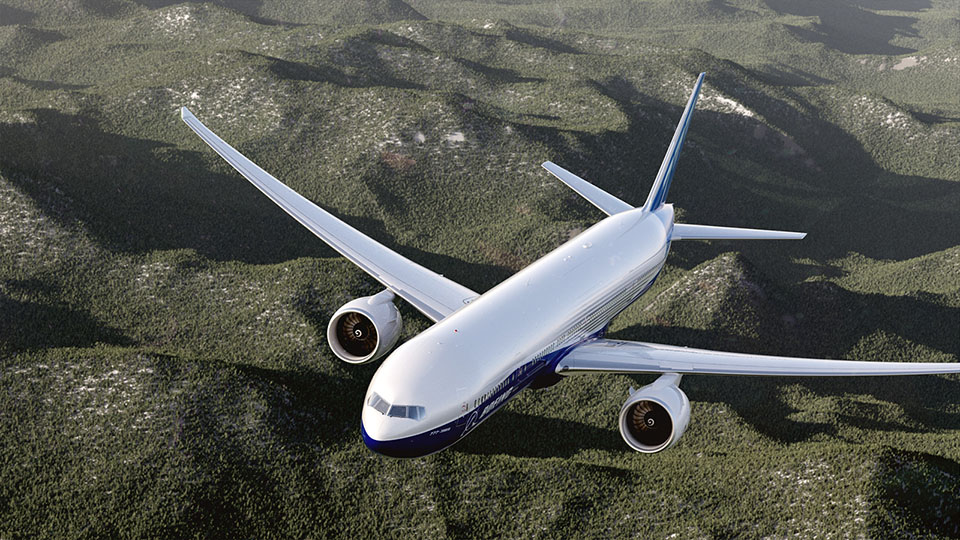
\includegraphics[width=1in]{img/plane-real.jpg}&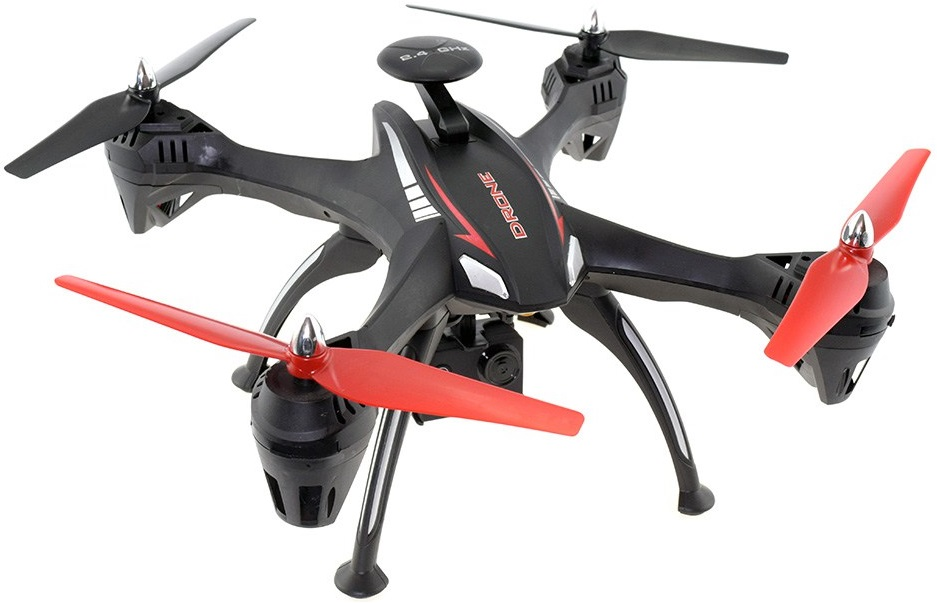
\includegraphics[width=1in]{img/quadcopter-real.jpg}&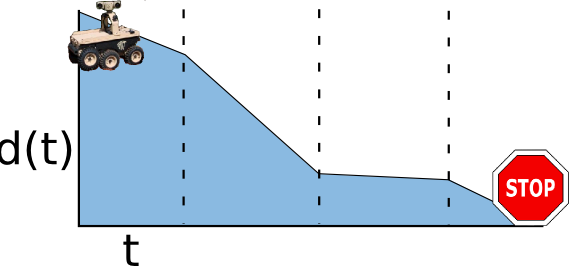
\includegraphics[width=1in]{img/robot-dyn-small.png}\\
Planes&Drones&Robots\\
\uncover<2->{
& &\\
%&$\Downarrow$&\\
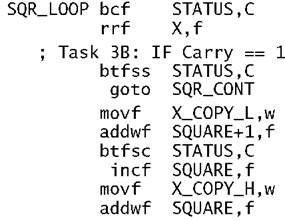
\includegraphics[width=0.6in]{img/assembly-small.png}&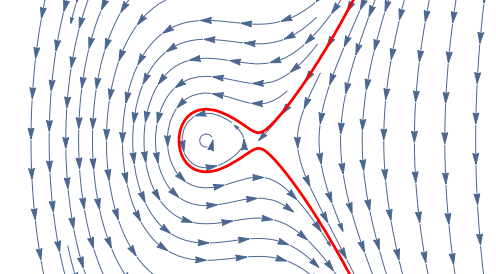
\includegraphics[width=1in]{img/invariant-region.png}&\infer{\Gamma \vdash A \land B}{\Gamma \vdash A}\\
Discrete Control & Continuous Dynamics & Syntactic Proof
}
    \end{tabular}
  \end{center}
  \only<1>{
  \begin{quote}
    How can we design cyber-physical systems people can bet their lives on? -- Jeanette Wing
  \end{quote}
  }
  \only<3>{
  \begin{quote}
    How do proofs cope when control, dynamics are partial, discontinuous?
  \end{quote}
  }
\end{frame}


\begin{frame}[t]{Verification Needs to be End-to-end}
  \begin{tabular}{lll}
%TODO: Make sure all systems are featured in intro pictures
%Pacemaker: 60k, Space shuttle: 400k, car: 100M, F22 > 1M, military drone >3M, 787: 14M, F35: 24M
%codebases
\ah{1}{Application}         & \ah{2}{Models LOC (approx.)}                      & \ah{3}{Real system LOC~\cite{codebases,OpenAPS}} \\
\acl{1}{Insulin pump}        & \acl{2}{30~\cite{COBELLI198227}}                   & \acl{3}{35K}  \\ % number of equations in pape
\acl{1}{Pacemaker}           & \acl{2}{650~\cite{DBLP:conf/cpsweek/AndalamMRT16}} & \acl{3}{60K}  \\ % 35 cells * 19 lines
\acl{1}{Space shuttle}       & \acl{2}{40~\cite{DBLP:conf/cpsweek/ChanM17}}       & \acl{3}{400K}\\ % artifact provided: spaceex
\acl{1}{Modern drone}        & \acl{2}{80~\cite{DBLP:conf/emsoft/RickettsML16}}   & \acl{3}{3M}\\
\acl{1}{Commercial airliner} & \acl{2}{84-150~\cite{DBLP:conf/fm/PlatzerC09,DBLP:conf/emsoft/JeanninGKGSZP15}} & \acl{3}{14M} \\  % tangential roundabout study, safe_explicit.kyx
\acl{1}{Modern car}          & \acl{2}{29-150~\cite{DBLP:conf/fm/LoosPN11,DBLP:journals/ral/BohrerTMSP19}}  & \acl{3}{100M} %FM kym3 proof, 
  \end{tabular}
\end{frame}

\begin{frame}[t]{End-to-end Verification Must Close Several Gaps}
Why are implementations more complicated than models?
  \begin{align*}
    \text{Learned Controls}   &\rightsquigarrow \text{Control envelopes}\\
    \text{Perception Systems} &\rightsquigarrow \text{Sensing assumptions}\\
    \text{Feedback Controls}  &\rightsquigarrow \text{Actuator assumptions}\\
    \text{Real physics}       &\rightsquigarrow \text{ODE Abstraction}\\
    \text{Non-critical code}  &\rightsquigarrow \langle\textbf{poof}\rangle
  \end{align*}
\end{frame}

\begin{frame}[t]{End-to-end Verification Must Meet Competing Needs}
  \begin{tabular}{lll}
    \ah{1}{\engineer} & \ah{2}{\logician} & \ah{3}{\logicuser}\\
    \acl{1}{Engineer} & \acl{2}{Logician} & \acl{3}{Logic-User}
  \end{tabular}
\end{frame}

\section{Related Work}
\begin{frame}[t]{General-purpose interactive theorem proving}
  \begin{tabular}{lll}
    \ah{1}{\engineer} & \ah{2}{\logician} & \ah{3}{\logicuser}\\
    \acl{1}{\saySad{Generated code is \\hard to integrate}} & \acl{2}{\sayHappy{Strong Foundations!}} & \acl{3}{\saySad{Long Proofs!}}
  \end{tabular}
  \begin{itemize}
  \item ROSCoq:~\cite{DBLP:conf/itp/AnandK15}       Coq proofs + control synthesis
  \item VeriDrone:~\cite{DBLP:conf/emsoft/RickettsML16}    LTL in Coq + monitor synthesis
  \item Isabelle/UTP:~\cite{DBLP:conf/utp/Foster19} CPS Embedded in Isabelle
  \end{itemize}
% Isabelle/Coq, VeriDrone, ROSCoq
\end{frame}

\begin{frame}[t]{Model Checking + Synthesis}
% LTLMoP, TuLiP, Seshia
  \begin{tabular}{lll}
    \ah{1}{\engineer} & \ah{2}{\logician} & \ah{3}{\logicuser}\\
    \acl{1}{\sayHappy{Synthesis tools!}} & \acl{2}{\saySad{Paper foundations}} & \acl{3}{\saySad{Hard models!}}
  \end{tabular}
  \begin{itemize}
  \item LTLMoP~\cite{DBLP:conf/iros/FinucaneJK10} and TuLiP~\cite{DBLP:conf/IEEEcca/FilippidisDLOM16}: Fancy front-end, synthesis via discretized model
  \item \cite{DBLP:conf/rv/DesaiDS17}: Constant dynamics, STL-based runtime monitor
  \item \cite{DBLP:conf/cdc/BhatiaKV10,DBLP:journals/automatica/FainekosGKP09}: Plan synthesis, complementary to control
  \end{itemize}
\end{frame}

\begin{frame}[t]{\dL Verification + Synthesis (before)}
  \begin{tabular}{lll}
    \ah{1}{\engineer} & \ah{2}{\logician} & \ah{3}{\logicuser}\\
    \acl{1}{\saySad{Limited synthesis}} & \acl{2}{\saySad{Paper foundations}} & \acl{3}{\saySad{Don't like tactics!}}
  \end{tabular}
  \begin{itemize}
  \item Uniform substitution~\cite[\S35,\S40]{Church:1956} is foundation of differential dynamic logic (\dL)~\cite{DBLP:journals/jar/Platzer17}
  \item \KeYmaeraX~\cite{DBLP:conf/cade/FultonMQVP15} prover uses Bellerophon~\cite{DBLP:conf/itp/FultonMBP17} language to express \dL proofs
  \item \ModelPlex~\cite{DBLP:journals/fmsd/MitschP16} synthesizes correct-by-construction monitor conditions from \dL model
  \end{itemize}
% dL, KeYmaera X, ModelPlex
\end{frame}

\begin{frame}[t]{No prior work meets all requirements}
\begin{table}[tbh]
  \centering
\begin{tabular}{l|c|c|r}
Approach    & Logician                 & Engineer                               & Logic-User\\\hline
GPITP       &\cellcolor{green!25}formal &\cellcolor{yellow!25}manual effort      &\cellcolor{orange!25}labor-intensive\\\hline
Automata    &\cellcolor{yellow!25}paper &\cellcolor{green!25}monitors, controls  &\cellcolor{orange!25}error-prone \\\hline
\dL before  &\cellcolor{yellow!25}paper &\cellcolor{yellow!25}some monitors      &\cellcolor{yellow!25}less error-prone\\\hline       %, less labor-intensive
\dL after   &\cellcolor{green!25}formal &\cellcolor{yellow!25}some monitors      &\cellcolor{yellow!25}less error-prone\\\hline\pause %, less labor-intensive
\CdGL       &\cellcolor{green!25}formal &\cellcolor{green!25}monitors, controls  &\cellcolor{green!25}least error-prone\\\hline       %, less labor-intensive
\end{tabular}
  \caption{Comparison of Verification Approaches}
  \label{tab:approach-comparison}
\end{table}
\end{frame}
\begin{frame}[t]{\CdGL Verification + Synthesis (after)}
  \begin{tabular}{lll}
    \ah{1}{\engineer} & \ah{2}{\logician} & \ah{3}{\logicuser}\\
    \acl{1}{\sayHappy{Full synthesis suite!}} & \acl{2}{\sayHappy{Formal foundations!}} & \acl{3}{\sayHappy{Structured proofs!}}
  \end{tabular}
\begin{tabular}{@{\hskip-0.2in}l@{\hskip-0.2in}l}
\begin{minipage}{0.6\textwidth}
{\small\begin{itemize}
  \item[] \textbf{Complete:} Formal soundness proof of \KeYmaeraX core
  \item[] \textbf{Complete:} Verified compilation for \ModelPlex monitors
  \item[] \textbf{Complete:} Logic for discrete games
\end{itemize}}
\end{minipage} &
\begin{minipage}{0.6\textwidth}
{\small\begin{itemize}
  \item[] \textbf{In-progress:} Structured proofs
  \item[] \textbf{Proposed:} Combined monitor, controller synthesis, via
  \item[] \textbf{Proposed:} Logic for hybrid games
\end{itemize}}
\end{minipage}
\end{tabular}

% dL, KeYmaera X, ModelPlex
\end{frame}


\section{Completed Work}
% Patter: We're now going to focus in on this thesis proper.
% First I'm going to discuss the completed works of the thesis, and for that I'm going to break
% down the thesis as a verification *pipeline*, as a series of steps in proof and implementation.
%
% Just to foreshadow: We will come back to the overview when I cover proposed work.
% The pipeline will be the same, rather the proposed work will achieve a better balance for our
% three characters within that pipeline.
\begin{frame}[t]{Approach of Thesis}
\begin{center}
  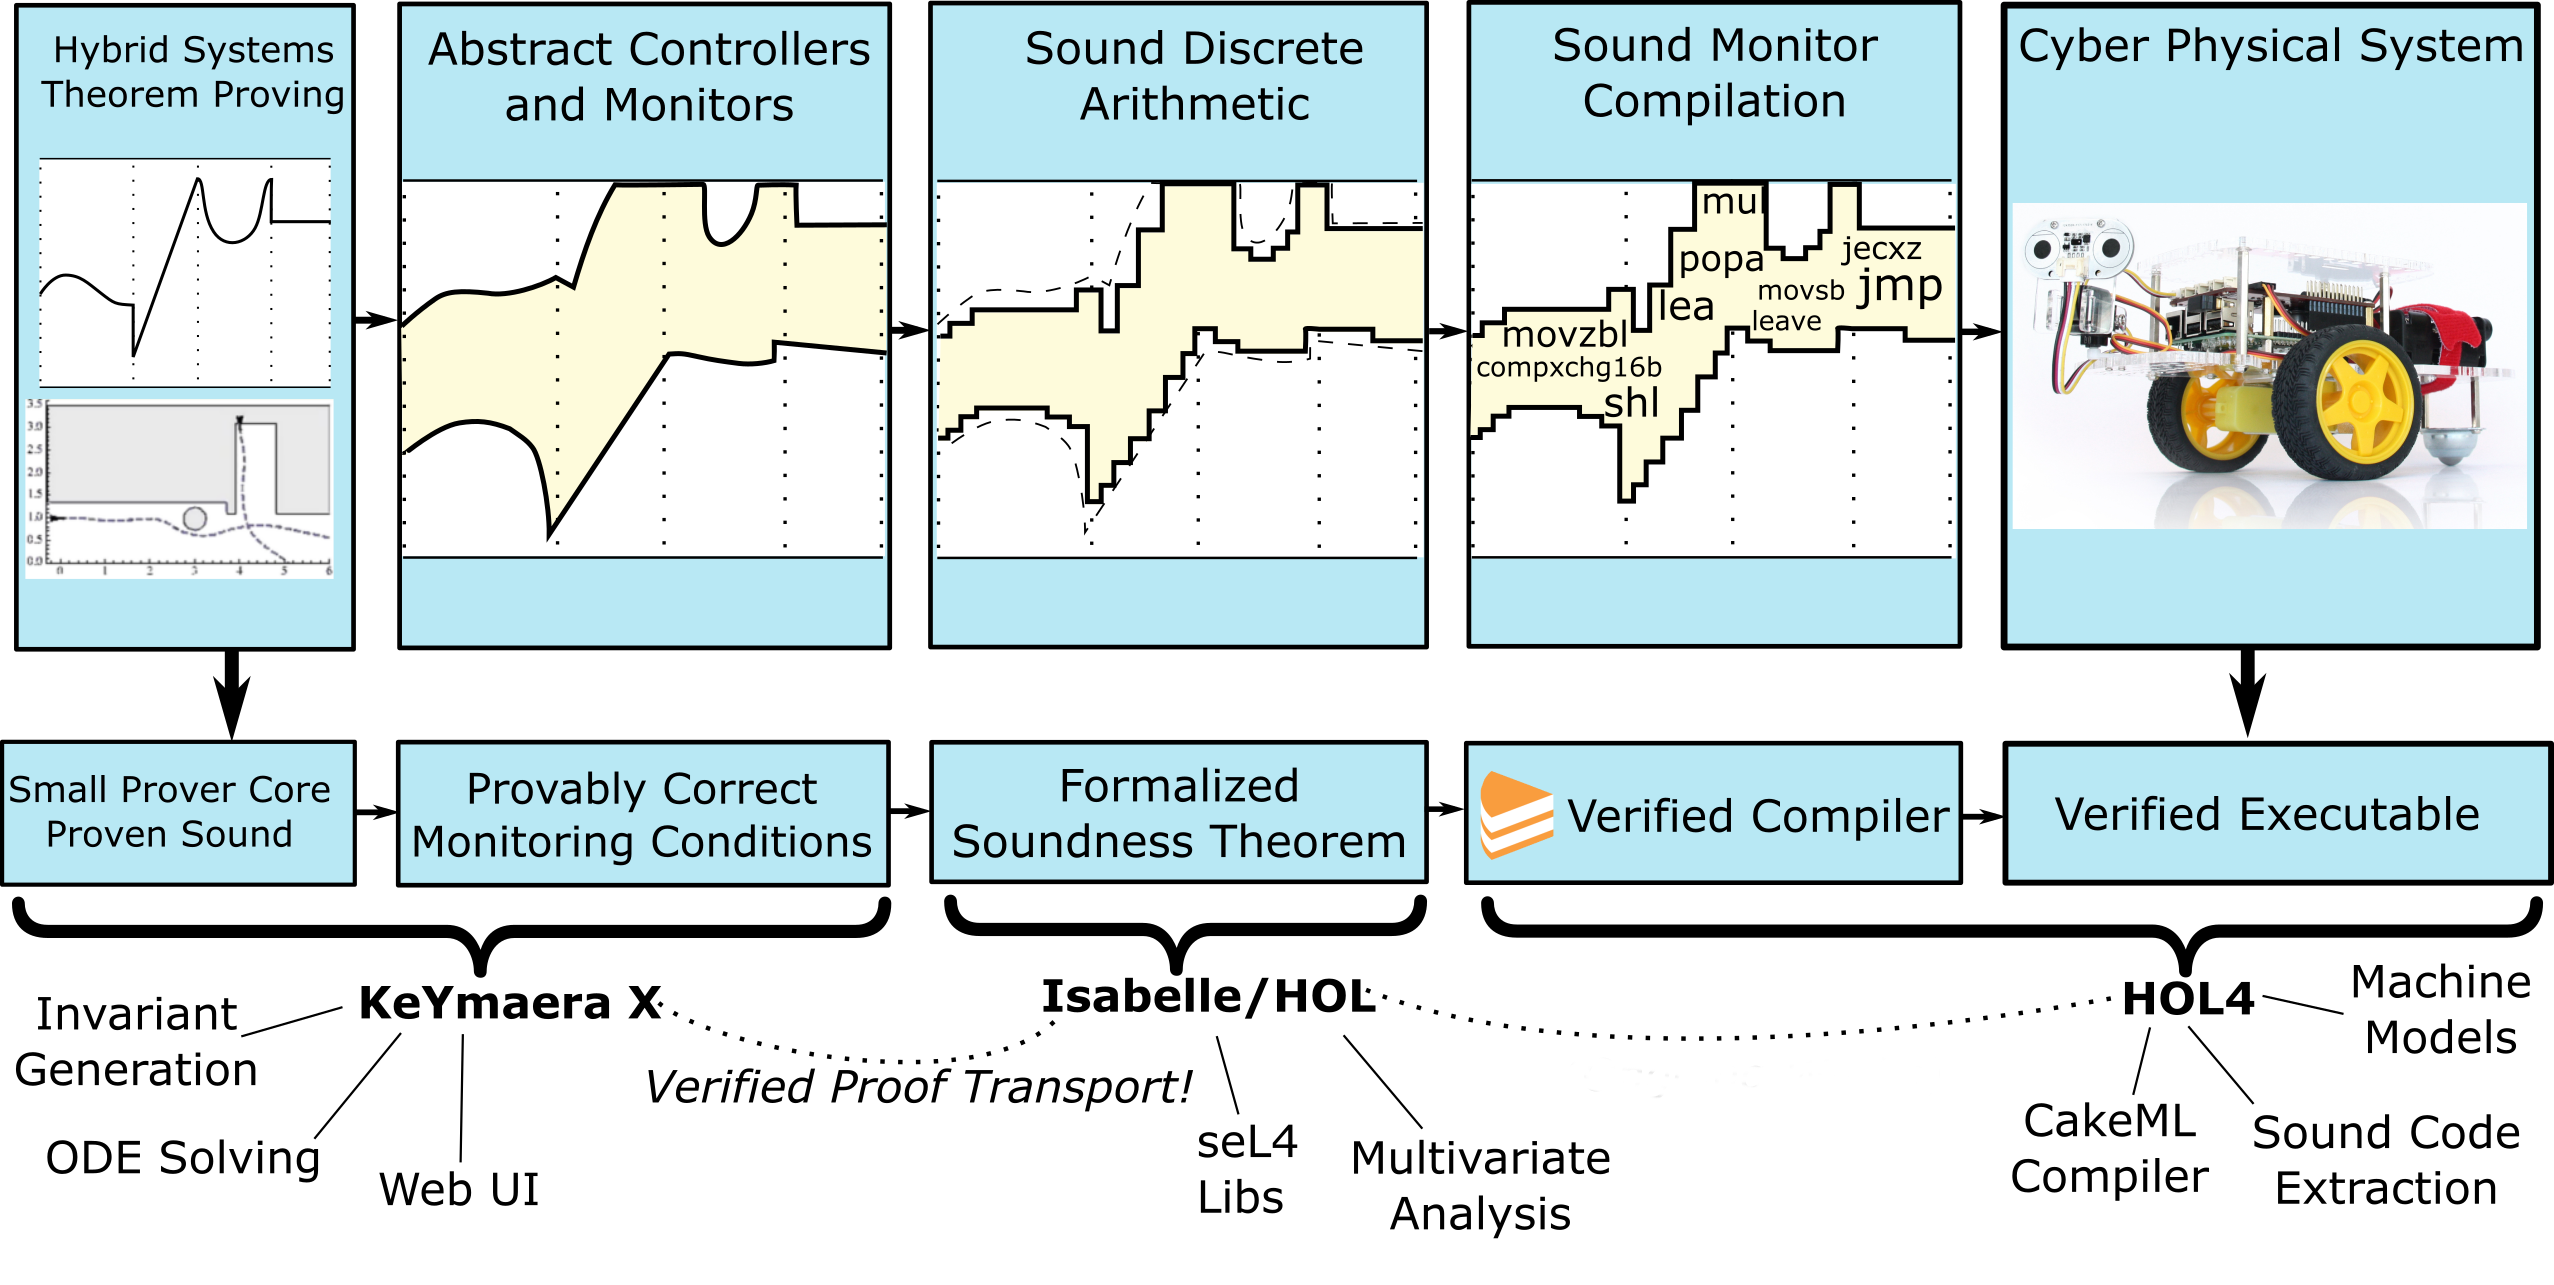
\includegraphics[width=4.4in]{img/veriphy-overview.png}
\end{center}
\end{frame}

\begin{frame}[t]{2D Driving Model is Source}
\newcommand{\admiss}{\textsf{Go}} % (\xgvar,\ygvar,\vlvar,\vhvar,\kvar,\avar)
\newcommand{\planreq}{\textsf{Feas}} % (\xgvar,\ygvar,\vlvar,\vhvar,\kvar,\avar)
\newcommand{\veps}{\varepsilon}
\newcommand{\annul}{\textsf{Ann}\xspace}
\newcommand{\adjustSpeedDist}{\delta_\mathsf{Lim}\xspace}
\newcommand{\controllableGoalDist}{\mathsf{Lim}}
{\small\begin{align*}
\ctrl &~\equiv~ \prandom{(\xgvar,\ygvar)};\,\prandom{[\vlvar,\vhvar]};\,\prandom{\kvar};\,\ptest{\planreq};\,\underbrace{\prandom{\avar};\,\ptest{\admiss}}_{\ctrlliv}\\
\annul &~\mequiv~\abs{\kvar}\veps \leq 1 \land \Big|\frac{ \kvar~\left(\xgvar^2 +\ygvar^2 - \veps^2 \right)}{2} - \xgvar\Big| < \veps\\
\label{eq:planReq} \planreq &~\equiv \annul \land \ygvar{>}0 \land 0{\leq}\vlvar{<}\vhvar \land \Avar\Tvar{\leq}\vhvar-\vlvar \land \Bvar\Tvar{\leq}\vhvar-\vlvar\\
\admiss &\equiv a \in [-B,A] \land safe(v(a,\veps),x(a,\veps))\\
\plant\equiv \{&\D{\xgvar}=-\vvar~\kvar~\ygvar,~\D{\ygvar}=\vvar~(\kvar~\xgvar-1),~\D{\vvar}=\avar,~\D{\tvar}=1 \\
 &\&~\tvar\leq \Tvar ~\land~ \vvar \geq 0\} %  ~\land~ yg > 0
\end{align*}}
% \end{align*}}       ~\hspace*{-5pt}


\end{frame}

%\begin{frame}[t]{Sandbox Safety Proof is Synthesized}
\begin{frame}[t]{Provable Monitor $\leadsto$ Provable Sandbox}
Sandboxed controller uses {\color{myyellow}{external}}  controller when decision is {\color{vred}safe}, else uses verified {\color{vgreen}{fallback}}.
Detects non-compliant {\color{vblue}plants}.
%\text{see \eqref{eq:ex-safetyprop}:}
% \text{see \eqref{eq:ex-safetyprop}}
\begin{textblock}{8}(1,3.5)
\small\begin{align*}
&\prandom{\vec{x}};\\
&\ptest{\phi}\\
& \bigl(\hspace{.5em} \color{myyellow}{\pumod{\vec{x}^+}{\textsf{extCtrl}}}\\
& \quad (~\phantom{\cup} \ptest{\color{vred}{\ctrlMon(\vec{x},\vec{x}^+)}}\\
& \quad \phantom{(~}\cup {\color{vgreen}{\fallback}} ~); \goback{}\\
& \quad \pumod{\vec{x}}{\vec{x}^+}\\
& \quad \prandom{\vec{x}^+} \\
& \quad  \ptest{\color{vblue}{\plantMon(\vec{x},\vec{x}^+)}};\\
& \quad  \pumod{\vec{x}}{\vec{x}^+}\bigr)^* 
  \end{align*}
\end{textblock}
\begin{textblock}{10}(5,3.5)
\small\begin{align*}
& \prandom{V};~\prandom{\varepsilon};~ \prandom{d};~\prandom{t}; \goback{}\\
& \ptest{d \geq 0 \land V\geq 0 \land \varepsilon \geq 0};  \goback{}\\
& \bigl(\hspace{.5em} \color{myyellow}{\prandom{t^+};~\prandom{v^+};~ \pumod{d^+}{d};}  \goback{}\\
& \quad (~\phantom{\cup} \ptest{\color{vred}{\ctrlMon(d,t,v,d^+,t^+,v^+)}}\\
& \quad \phantom{(~}\cup \color{vgreen}{\pumod{t^+}{0};~\pumod{v^+}{0}} ~); \goback{}\\
& \quad \pumod{t}{t^+};~\pumod{v}{v^+};  \goback{}\\
& \quad  \prandom{d^+};~\prandom{t^+};  \goback{}\\
& \quad  \ptest{\color{vblue}{\plantMon(d,t,v,d^+,t^+,v^+)}};\\
& \quad  \pumod{d}{d^+};~\pumod{t}{t^+}  \goback{}\bigr)^* 
\end{align*}
\end{textblock}
\end{frame}

\begin{frame}[t]{Proof Term is Cross-Checked}
How to trust a theorem prover?
Formalize it!
\Isabelle function \texttt{pteval} computes the proof state proved by a given proof term, or returns \texttt{NONE} on proofs that do not check
\[{\tt pteval} : {\tt pt} \to {\tt proofState\ option}\]
\KeYmaeraX is instrumented with a proofterm checker.
The synthesized checker was evaluated on a 100,000-step sandbox safety proof.
\end{frame}

\begin{frame}[t]{Cross-checker is Verified}
Decidable first-order arithmetic is assumed ``axiomatically,'' all other rules are proven sound.
\begin{theorem}[Proof-checker soundness]
If all real arithmetic subgoals are valid and the proof checker accepts the proof term, the output derived rule is sound, i.e.:
\[\small\texttt{arith\_valid pt} \land \texttt{pteval\ pt = Some rule} \limply \texttt{sound(rule)}\]
\end{theorem}
\end{frame}

\begin{frame}{Sandbox is Discretized}
\textbf{Example:} Check whether $\pi < e$, efficiently.\\
\textbf{Solution:} Conservative interval approximation
\begin{example}
Let $\nu_I=\{pi\mapsto[3,4],e\mapsto[2,3]\}$, then 
\begin{itemize}
%\item<+-> \(pi <_w e\) is false ($\bot$)\hspace{1.16in}\includegraphics[width=1.5in]{img/
\item<+-> \(pi <_w e\) is false ($\bot$)\hspace{1.63in}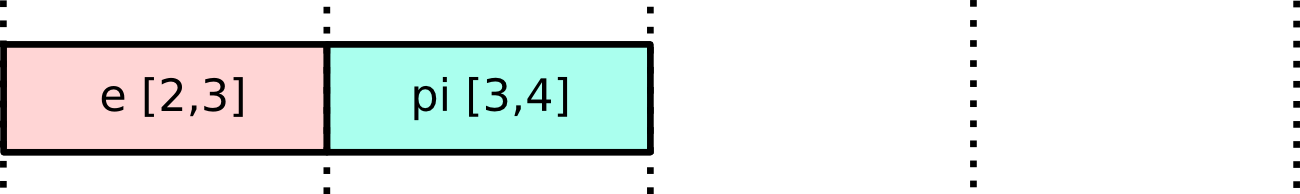
\includegraphics[width=1.875in]{img/interval1.png}
\item<+-> \(pi <_w e + 3\) is true ($\top$)\hspace{1.4in}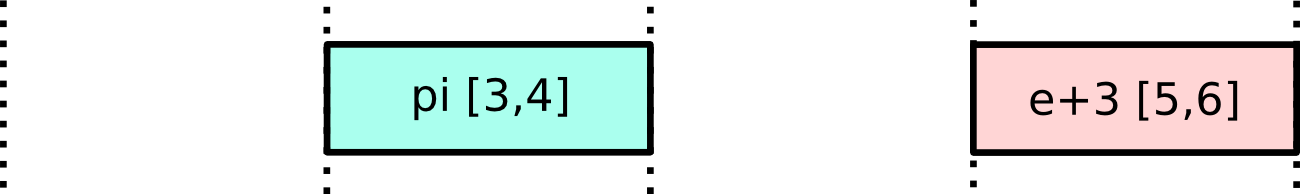
\includegraphics[width=1.875in]{img/interval2.png}
\item<+-> \(pi <_w e + 1\) is \emph{a known unknown} ($U$){\hspace{0.50875in}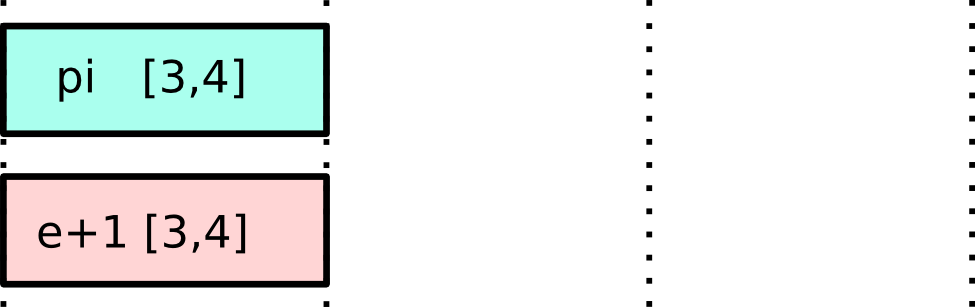
\includegraphics[width=1.40625in]{img/interval3.png}}
\end{itemize}
\only<4>{When truth values can be unknown, resulting logic is \emph{3-valued}}
\end{example}
\begin{textblock}{10}(14,1.75)
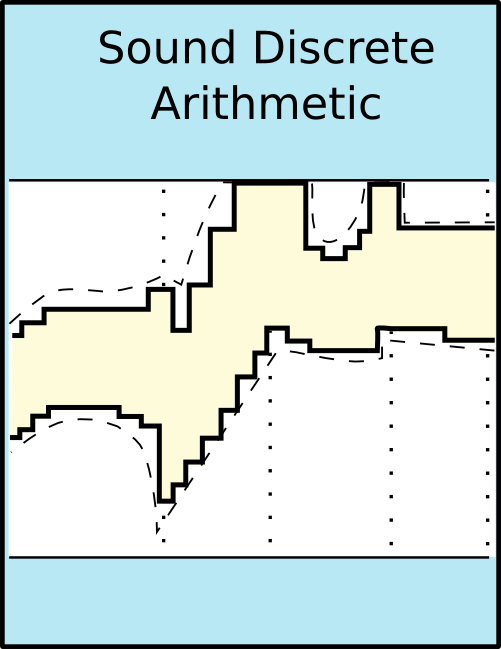
\includegraphics[width=0.7in]{img/focus-int.png}
\end{textblock}
\end{frame}

\begin{frame}[t]{Discrete Sandbox is Compiled}
  \CakeML source incorporates {\color{myyellow}{external}} control, actuation, sensing
\footnotesize\begin{align*}
\textbt{fun}&~\texttt{cmlSandbox state =}\short
&\textbt{if}~\texttt{not ({\color{myyellow}stop ()}) }\textbt{then}\short
&\quad\texttt{state.ctrl}^+ \texttt{:= {\color{\extern}extCtrl state};}\short
&\quad\texttt{state.ctrl := }\textbt{if}\texttt{ {\color{vred}intervalSem ctrlMon state}} = \top \short
&\quad\quad\qquad\qquad\qquad\textbt{then}\texttt{ state.ctrl}^+\short
&\quad\quad\qquad\qquad\qquad\textbt{else}\texttt{ {\color{vgreen}fallback state;}}\short
&\quad\texttt{{\color{\extern}actuate state.ctrl};}\short
&\quad\texttt{state.sensors}^+\texttt{:= {\color{\extern}sense ()};}\short
&\quad\textbt{if}\texttt{ {\color{vblue}intervalSem plantMon state}} = \top\texttt{ }\textbt{then} \short
&\quad\quad\texttt{Runtime.fullGC ();} \short
&\quad\quad\texttt{state.sensors := state.sensors}^+\texttt{;} \short
&\quad\quad\texttt{cmlSandbox state} \short
&\quad\textbt{else}\texttt{ violation "Plant Violation"}
\end{align*}
\end{frame}

\begin{frame}[t]{Compiled Code is Simulated}
\begin{figure}[tb]
\centering
\begin{minipage}[b]{2in}\centering
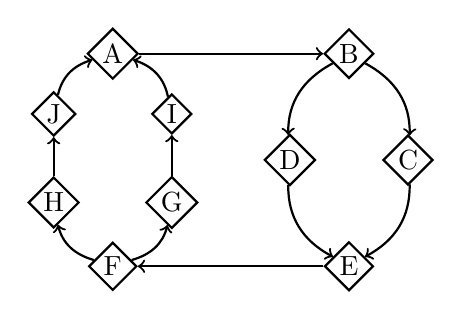
\begin{tikzpicture}[->,draw,thick,yscale=0.9,inner sep=1pt]
\tikzstyle{arc}=[circle,draw]
\tikzstyle{line}=[rectangle,draw]
\tikzstyle{way}=[diamond,draw]
\node[way] (a) at (1,3) {A};
\node[way] (b) at (4,3) {B};
\node[way] (c) at (4.75,1.5) {C};
\node[way] (d) at (3.25,1.5) {D};
\node[way] (e) at (4,0) {E};
\node[way] (f) at (1,0) {F};
\node[way] (g) at (1.75,0.90) {G};
\node[way] (h) at (0.25,0.90) {H};
\node[way] (i) at (1.75,2.15) {I};
\node[way] (j) at (0.25,2.15) {J};
\draw (a) -> (b);
\draw (b) edge [bend left] node {} (c);
\draw (b) edge [bend right] node {} (d);
\draw (c) edge [bend left]node {} (e);
\draw (d) edge [bend right] node {} (e);
\draw (e) -> (f);
\draw (f) edge [bend left]  node {} (h);
\draw (f) edge [bend right] node {} (g);
\draw (h) -> (j);
\draw (g) -> (i);
\draw (j) edge [bend left]  node {} (a);
\draw (i) edge [bend right] node {} (a);
\end{tikzpicture}
\subcaption{Example mission}\label{fig:patrol-mission-plan}\end{minipage}
\begin{minipage}[b]{1.51in}\centering
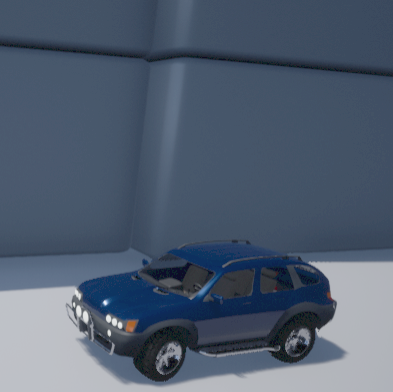
\includegraphics[width=1.51in,clip,trim=0 0 0 50]{graphics/airsim.png}
\subcaption{Simulator}\label{fig:simulator}\end{minipage}
%\begin{minipage}[b]{.3\linewidth}\centering
%\includegraphics[width=1.95in]{graphics/robot.jpg}
%\subcaption{RC car}\label{fig:rccar}
%\end{minipage}
\begin{minipage}[b]{1in}\centering
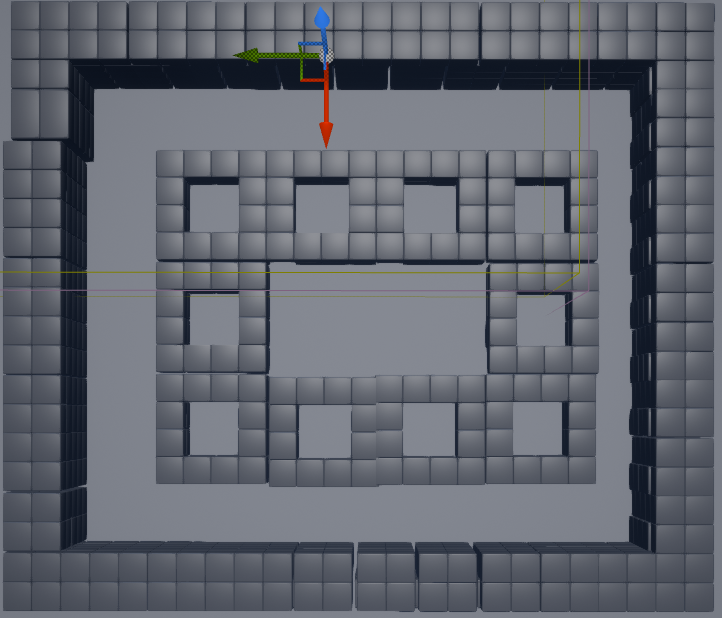
\includegraphics[width=1in]{graphics/screen1.png}
\subcaption{Rectangle}\label{fig:rect}\end{minipage}\\
\begin{minipage}[b]{1in}\centering
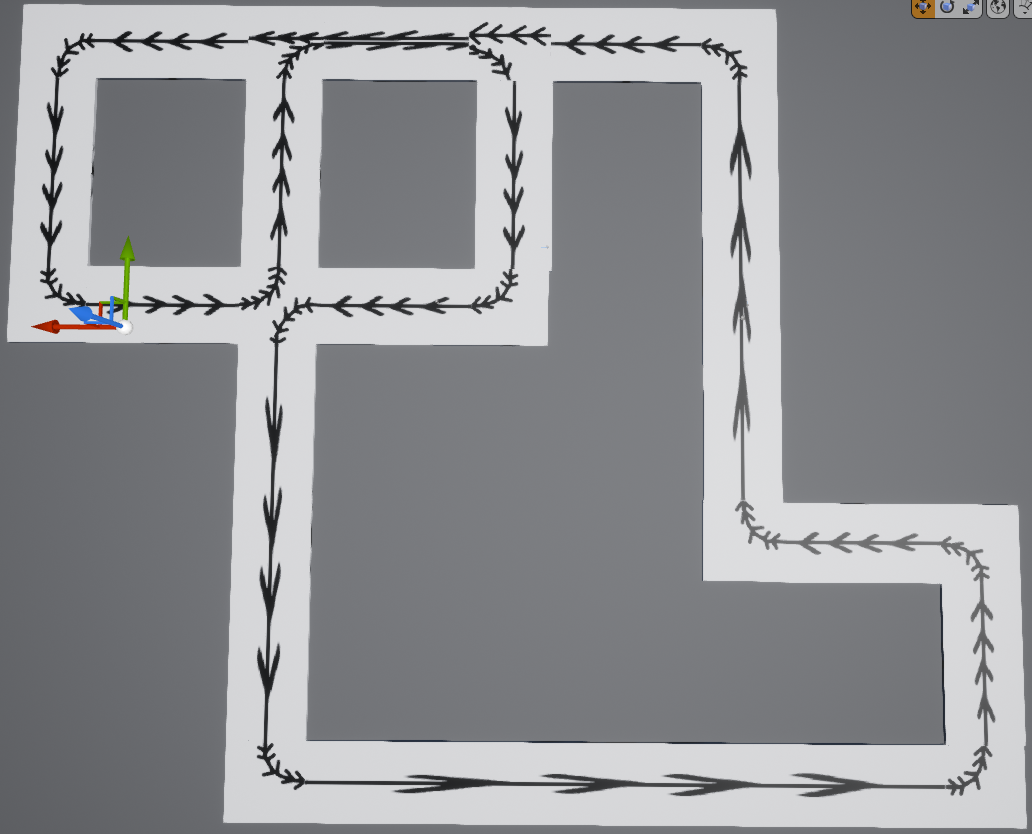
\includegraphics[width=1in]{graphics/screen2.png}
\subcaption{Tight turns}\label{fig:turns}\end{minipage}
\begin{minipage}[b]{1in}\centering
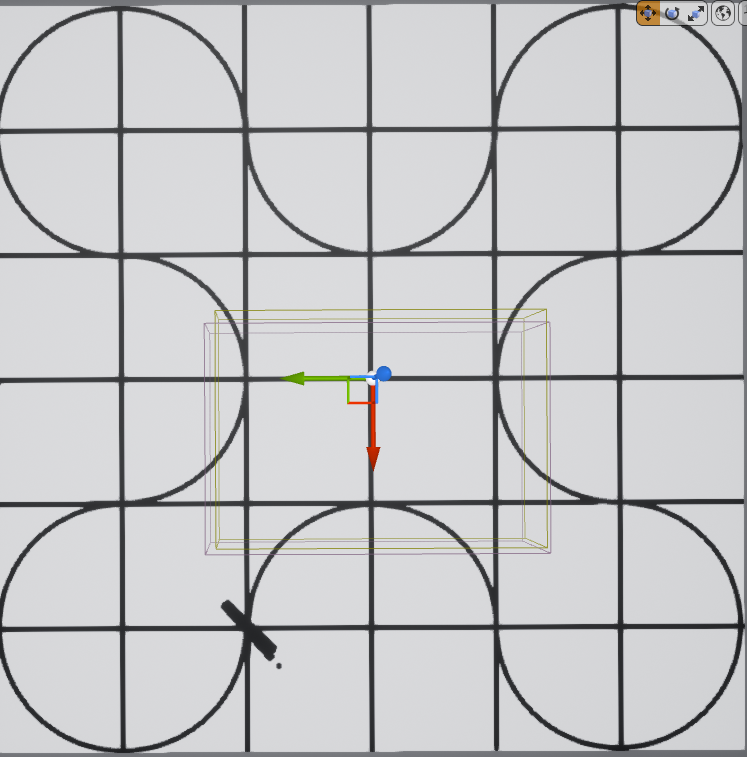
\includegraphics[width=0.8in]{graphics/screen3.png}
\subcaption{Large clover}\label{fig:clover}\end{minipage}
\caption{Implementation and environments built in AirSim}
\label{fig:patrol-plan}
\end{figure}

\end{frame}

\newcommand{\ctrlspike}{\Large{\bf C\dag}}
\newcommand{\ctrlfault}{\Large{\bf C\Lightning}}
\newcommand{\plantfault}{\Large{\bf P\Lightning}}
\newcommand{\ctrlrestore}{\Large{\bf C\tiny\Checkmark}}
\newcommand{\graphscale}{0.4}
\newcommand{\obsforward}{\Large{\bf{Ob{+}}}}
\newcommand{\obsback}{\Large{\bf{Ob{-}}}}
\newcommand{\obshalt}{\Large{\bf{Ob{0}}}}
\newcommand{\graphwidth}{6.5in}
\newcommand{\graphheight}{8.5cm}
\begin{frame}[t]{Code Executed on GoPiGo Robot}
\begin{textblock}{8}(1.9,2.7)
Operational Suitability? \\
Arithmetic Precision?    
\end{textblock}
\begin{textblock}{8}(12,2)
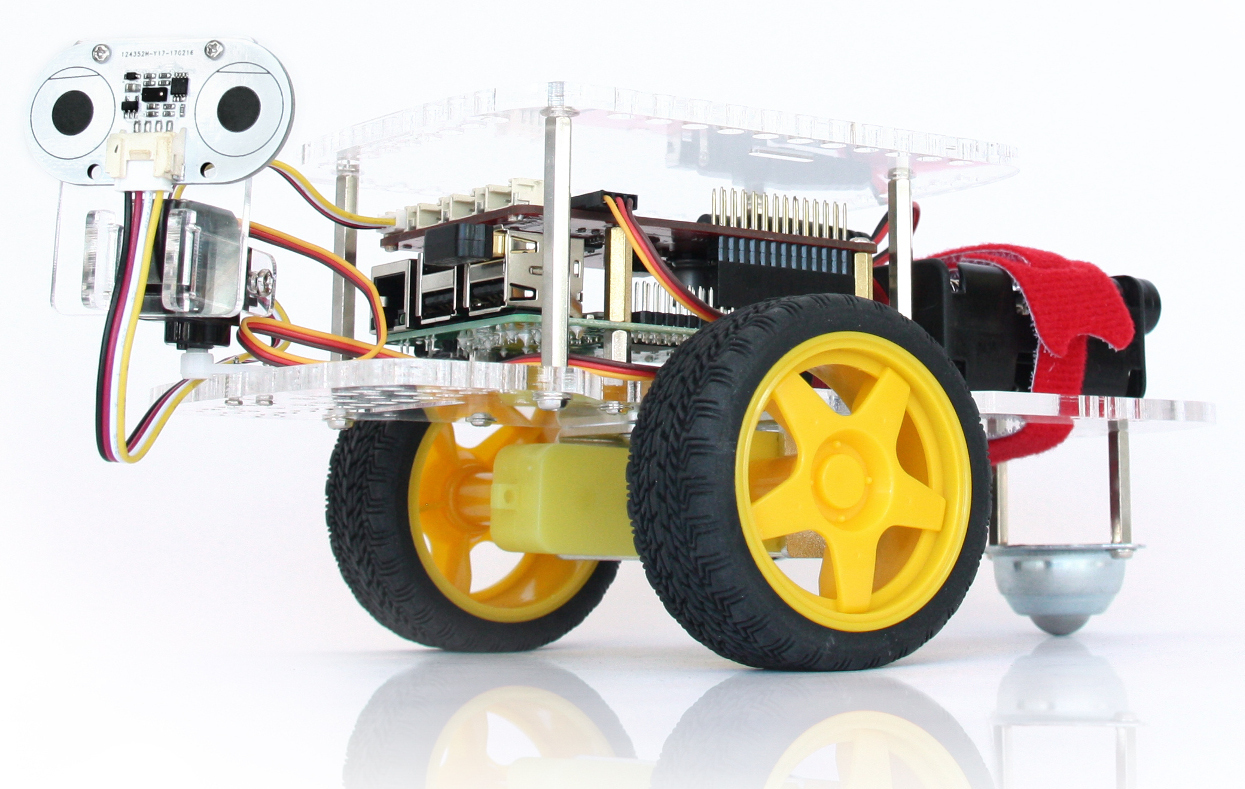
\includegraphics[width=1.2in]{img/gopigo3.jpg}\\
\end{textblock}
%  \begin{itemize}[<+->]
%  \item Invariants from proof essential 
%  to avoid false alarms
%  \item Arithmetic precision was sufficient
%  \item Monitors catch model deviations
%  \item Monitors were not overly conservative
%  \end{itemize}
\begin{textblock}{100}(1,5.2)
    \begin{tabular}{lr}
\begin{tikzpicture}[trim axis left,scale=\graphscale]
      \begin{axis}[ scale only axis, width=\graphwidth, height=\graphheight,
        ytick scale label code/.code={}, xtick scale label
        code/.code={}, scaled x ticks=base 10:-3, scaled y ticks=base
        10:-4, x label style={at={(axis description
            cs:1.03,0)},anchor=north east}, xlabel={time
          $[\textit{s}]$}, y label style={at={(axis description
            cs:0,1.0)},rotate=-90,anchor=south west},
        ylabel={distance $[\textit{cm}]$}, grid=both, axis on top,
        cycle list name=auto, clip=false, enlargelimits=false, legend style={at={(0.95,0.95)}}]
        \addplot+[myblue,mark=,solid,ultra thick]
        table[x=time,y=d,skip first n=1,col sep=comma]
        {correct100.csv};
        \addlegendentry{Controller A (correct)};
        % \node[coordinate,pin={[align=center,pin
        % distance=2cm]86:{\Lightning~Fault becomes\\
        % safety-critical,\\ fallback engaged}}] at (axis
        % cs:4400,46000) {};
        \coordinate (fault1) at (axis cs:4400,46000);
        \addplot+[vgreen,mark=,ultra thick] table[x=time,y=d,skip
        first n=1,col sep=comma]
        {ctrlbug100.csv};
        \addlegendentry{Controller B (faulty)};
        % \coordinate (fault1) at (axis cs:4400,46000);
        \node[coordinate,pin={[align=center,pin
          distance=0.5cm]90:{\textcolor{vgreen}{\ctrlspike}}}] at
        (axis cs:2700,460000) {};
        \addplot+[myyellow,mark=,dashed,ultra thick]
        table[x=time,y=d,skip first n=1,col sep=comma]
        {backwards100.csv};
        \addlegendentry{Malicious obstacle};
        % \node[coordinate,pin={[align=center,pin
        % distance=0.5cm]130:{\Lightning~Fault becomes\\
        % safety-critical,\\ fallback engaged}}] at (axis
        % cs:3300,24000) {};
        \coordinate (fault2) at (axis cs:3300,24000) {};
        \node[coordinate,pin={[align=center,pin
          distance=0cm]180:{\textcolor{myyellow}{\ctrlspike}}}] at
        (axis cs:1900,450000) {}; \node[coordinate,pin={[pin
          distance=0cm]260:{\textcolor{myyellow}{\plantfault}}}] at
        (axis cs:3740,2000) {};
        % BB%\node[coordinate,pin=below left:{\plant violation}] at (axis cs:3740,2000) {};
        \addplot+[black,mark=,ultra thick] table[x=time,y=d,skip first
        n=1,col sep=comma]
        {actoffsetSafe100.csv};
        \addlegendentry{Small disturbance};
        % \node[coordinate,pin={[align=center,pin
        % distance=1cm]60:{\Lightning~Fault becomes\\
        % safety-critical,\\ fallback engaged}}] at (axis
        % cs:5060,19600) {};
        \coordinate (fault3) at (axis cs:5060,19600) {};
        \node[coordinate,pin={[align=center,pin
          distance=0cm]70:{\textcolor{black}{\ctrlspike}}}] at (axis
        cs:2860,492600) {}; %(axis cs:2640,486000) {};
        \node[coordinate,pin={[align=center,pin
          distance=0.2cm]120:{\ctrlrestore}}] at (axis cs:8800,57000)
        {}; \node[coordinate,pin={[align=center,pin
          distance=0.2cm]205:{\ctrlfault}}] at (axis cs:9020,4200) {};
        % Fault again\\ safety-critical,\\
        % \coordinate (fault4) at (axis cs:9020,4200) {};
        \addplot+[myblue,mark=,dashed,ultra thick]
        table[x=time,y=d,skip first n=1,col sep=comma]
        {actoffsetUnsafe100.csv};
        \addlegendentry{Large disturbance};
        \node[coordinate,pin={[align=center,pin
          distance=0cm]180:{\textcolor{myblue}{\ctrlspike}}}] at (axis
        cs:2600,450000) {}; \node[coordinate,pin={[align=center,pin
          distance=0cm]160:{\textcolor{myblue}{\ctrlfault}}}] at (axis
        cs:4200,3000) {};
        % Fault becomes\\ safety-critical,\\
        % BB%\node[coordinate,pin={[align=center,pin distance=1.2cm]265:{\Lightning~Fallback engages}}] (faulttext) at (axis cs:4400,24000) {};

        \node[coordinate,pin={[align=center,pin
          distance=0cm]270:{\textcolor{myblue}{\plantfault}}}] at
        (axis cs:6600,2000) {};
        \node[coordinate,pin={[align=center,pin distance=0.2cm]20:{\textcolor{vgreen}{\ctrlfault}}}] at (fault1) {};
        \node[coordinate,pin={[align=center,pin
          distance=0cm]180:{\textcolor{myyellow}{\ctrlfault}}}] at
        (fault2) {}; \node[coordinate,pin={[align=center,pin
          distance=0cm]240:{\textcolor{black}{\ctrlfault}}}] at
        (fault3) {};
        % \draw[-,thin] (fault1) -- ($(faulttext)+(-0.9cm,-1.2cm)$);
        % \draw[-,thin] (fault2) -- ($(faulttext)+(-0.9cm,-1.2cm)$);
        % \draw[-,thin] (fault3) -- ($(faulttext)+(-0.9cm,-1.2cm)$);
      \end{axis}
    \end{tikzpicture}
&\vspace{-0.8cm}
\begin{tikzpicture}[trim axis left,scale=\graphscale]
\begin{axis}[
scale only axis,
width=\graphwidth,
height=\graphheight,
ytick scale label code/.code={},
xtick scale label code/.code={},
scaled x ticks=base 10:-3,
scaled y ticks=base 10:-4,
x label style={at={(axis description cs:1.03,0)},anchor=north east},
xlabel={time $[\textit{s}]$},
y label style={at={(axis description cs:0,1)},rotate=-90,anchor=south west},
ylabel={distance $[\textit{cm}]$},
grid=both,
axis on top,
cycle list name=auto,
clip=false,
enlargelimits=false,
legend style={at={(0.95,0.95)}}
%legend style={at={(0.98,1.1)}}
]
 \addplot+[myblue,mark=,ultra thick] table[x=time,y=d,skip first n=0,col sep=comma] {sim/correct100.csv};
\addlegendentry{Controller A (correct)};
%\node[coordinate,pin={[align=center,pin distance=2cm]86:{\Lightning~Fault becomes\\ safety-critical,\\ fallback engaged}}] at (axis cs:4400,46000) {};
 \addplot+[vgreen,mark=,ultra thick] table[x=time,y=d,skip first n=0,col sep=comma] {sim/ctrlbug100.csv};
\addlegendentry{Controller B (faulty)};
\node[coordinate,pin={[align=center,pin distance=0.1cm]70:{\textcolor{vgreen}{\ctrlspike}}}] at (axis cs:2445,460000) {};
% Fault becomes\\ safety-critical,\\ f
\node[coordinate,pin={[align=center,pin distance=-0.1cm]45:{\textcolor{vgreen}{\ctrlfault}}}] at (axis cs:4109,46000) {};
 \addplot+[myyellow,mark=,ultra thick] table[x=time,y=d,skip first n=0,col sep=comma] {sim/backwards100.csv};
\addlegendentry{Approaching obstacle};
\node[coordinate,pin={[align=center,pin distance=0.2cm]265:{\textcolor{myyellow}{\obsforward}}}] at (axis cs:2074,422000) {};
\node[coordinate,pin={[align=center,pin distance=0cm]-70:{\textcolor{myyellow}{\obsback}}}] at (axis cs:4295,18000) {};
\node[coordinate,pin={[align=center,pin distance=0cm]-0:{\textcolor{myyellow}{\obshalt}}}] at (axis cs:5774,486000) {};
\addplot+[black,mark=,ultra thick] table[x=time,y=d,skip first n=0,col sep=comma] {sim/forwardObstCompensatesUnsafeActoffset100.csv};
\addlegendentry{Robot follows obstacle};
\node[coordinate,pin={[align=center,pin distance=0.2cm]86:{\obsforward}}] at (axis cs:5218,214000) {};
\end{axis}
\end{tikzpicture}
    \end{tabular}
\end{textblock}
\renewcommand{\ctrlspike}{\small{\bf C\dag}}
\renewcommand{\ctrlfault}{\small{\bf C\Lightning}}
\renewcommand{\plantfault}{\small{\bf P\Lightning}}
\renewcommand{\ctrlrestore}{\small{\bf C\tiny\Checkmark}}
\renewcommand{\obsforward}{\small{\bf{Ob{+}}}}
\renewcommand{\obsback}{\small{\bf{Ob{-}}}}
\renewcommand{\obshalt}{\small{\bf{Ob{0}}}}

\begin{textblock}{100}(3,12.5)
Control Fault \ctrlfault{}, Plant Fault \plantfault{}, Control Spike \ctrlspike{}, Obstacle Motion {\textbf{Ob}}
\end{textblock}
\end{frame}

% https://github.com/jsford/FFAST
\begin{frame}[t]{More Hardware Platforms Available}
Several hardware platforms are available through collaborators if needed for further evaluation:
\begin{itemize}
\item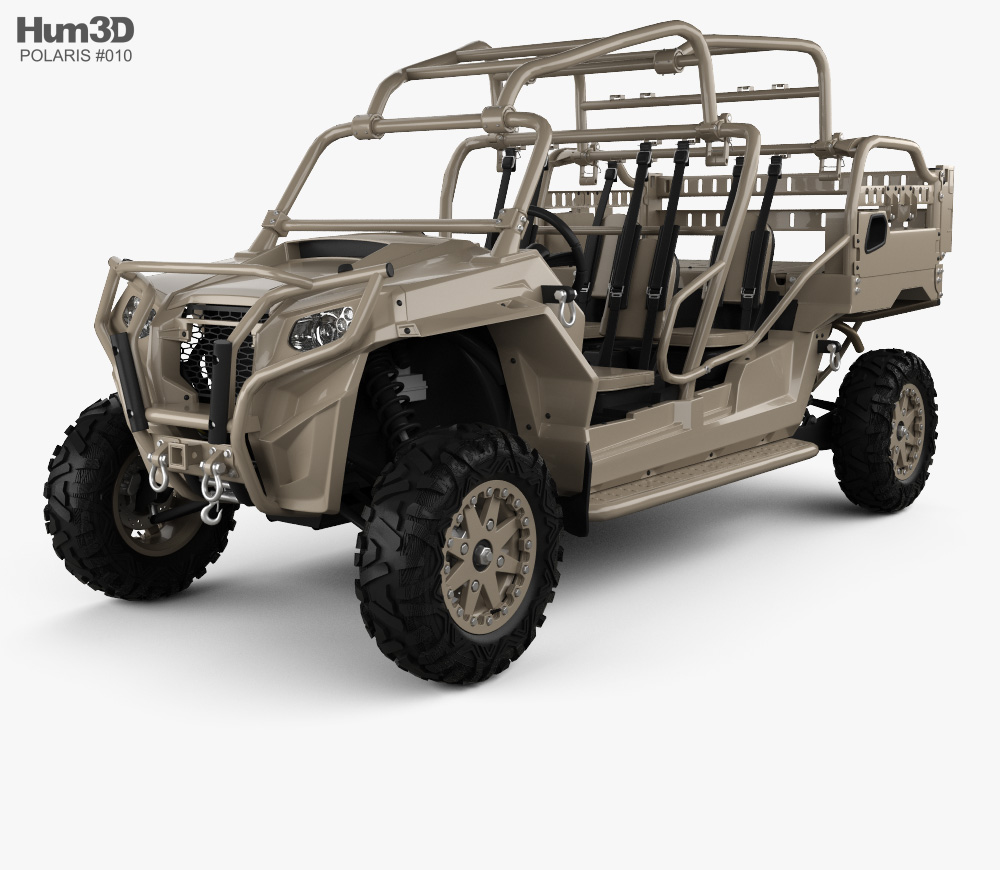
\includegraphics[width=1.2in]{img/mrzr.jpg}\\
Polaris MRZR (access on limited dates only)
\item 1-10th scale RC Car (full access)
\end{itemize}

\end{frame}

%\begin{minipage}[b]{2in}
\begin{frame}[t]{Components of Thesis}
%\begin{figure}[tbh]
%  \centering
\begin{center}
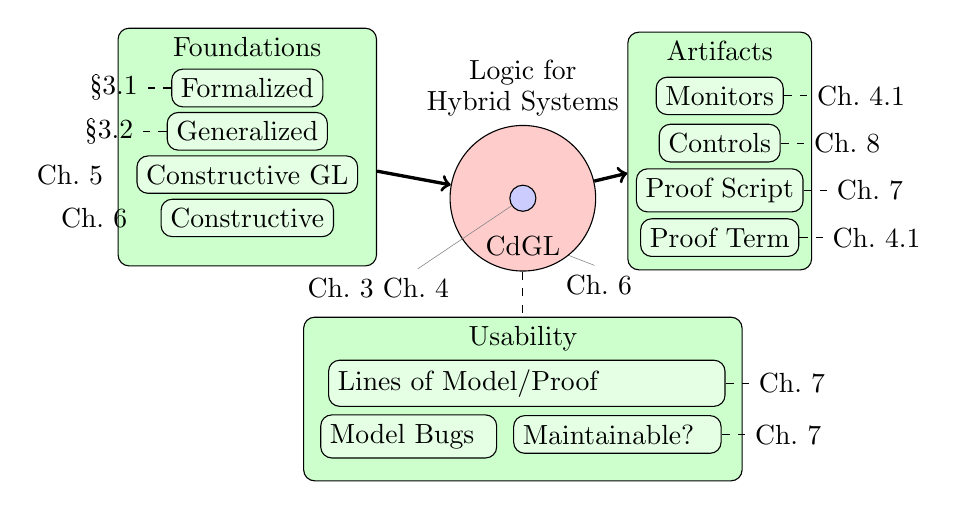
\begin{tikzpicture}[scale=0.5]
\draw (0,3.2)  node {Logic for};
\draw (0,2.4)  node {Hybrid Systems};
\draw (0,0)   node[circle]      (CdGLcirc) {\phantom{\hspace{1.1cm}}};
\draw (0,-1) node (cdgl) {\phantom{\CdGL}};
\node[coordinate,pin={[pin distance=0.55cm,text width=2cm]320:{Ch.\ 6}}] (cdgl-ref) at (cdgl) {};
\draw (0,0)   node[circle, fill=red!20,draw]      (CdGLcirc) {\phantom{\hspace{1.6cm}}};
\draw (0,-1.2) node (cdgl) {\CdGL};
\draw (0,0)   node[circle]  (dl)  {\phantom{\dL}};
\node[coordinate,pin={[pin distance=0.9cm,text width=3cm]265:{\ \ \ \ Ch.\ 3 Ch.\ 4}}] (dl-ref) at (dl) {};
\draw (dl) node[circle, fill=blue!20,draw]  {\dL};
\draw (-7, 1.3) node[rectangle,rounded corners,fill=green!20,draw,text depth=1in,text width=1.2in,text centered] (logic) {Foundations};
\draw (-7, 2.8) node[rectangle,rounded corners,fill=green!10,draw,thin,minimum height=0.3cm] (formalization) {\dL Formalized};
\draw (-7, 1.7) node[rectangle,rounded corners,fill=green!10,draw,thin,minimum height=0.3cm] (generalization) {\dL Generalized};
\draw (-7, 0.6) node[rectangle,rounded corners,fill=green!10,draw,thin,minimum height=0.3cm] (cgl) {Constructive \GL};
\draw (-7, -0.5) node[rectangle,rounded corners,fill=green!10,draw,thin,minimum height=0.3cm] (cdgl) {Constructive \dGL};
\draw node[left=0.3cm of formalization] (formal-ref) {\S3.1};
\draw node[left=0.3cm of generalization] (gen-ref) {\S3.2};
\draw node[left=0.3cm of cgl] (cgl-ref) {Ch.\ 5};
\draw node[left=0.3cm of cdgl] (cdgl-ref) {Ch.\ 6};
\draw[dashed] (formalization) -- (formal-ref);
\draw[dashed] (generalization) -- (gen-ref);
\draw (5, 1.2) node[rectangle,rounded corners,fill=green!20,draw,text depth=1in,text width=2.1cm,text centered] (engine) {Artifacts};
\draw (5, 2.6) node[rectangle,rounded corners,fill=green!10,draw,thin,minimum height=0.3cm] (monitors) {Monitors};
\draw (5, 1.4) node[rectangle,rounded corners,fill=green!10,draw,thin,minimum height=0.3cm] (controllers) {Controls};
\draw (5, 0.2) node[rectangle,rounded corners,fill=green!10,draw,thin,minimum height=0.3cm] (proofscript) {Proof Script};
\draw (5, -1) node[rectangle,rounded corners,fill=green!10,draw,thin,minimum height=0.3cm] (proofterm) {Proof Term};
\draw node[right=0.3cm of monitors] (monitor-ref) {Ch.\ 4.1};
\draw node[right=0.3cm of controllers] (controllers-ref) {Ch.\ 8};
\draw node[right=0.3cm of proofscript] (proofscript-ref) {Ch.\ 7};
\draw node[right=0.3cm of proofterm] (proofterm-ref) {Ch.\ 4.1};
\draw[dashed] (monitors) -- (monitor-ref);
\draw[dashed] (controllers) -- (controllers-ref);
\draw[dashed] (proofscript) -- (proofscript-ref);
\draw[dashed] (proofterm) -- (proofterm-ref);
\node[shape=coordinate] (use-anchor) at (0,-3){};
%\draw (1.45,-2) -- (0,-2.7);
\draw (0, -5.1) node[rectangle,rounded corners,fill=green!20,draw,text depth=1.6cm,text width=2.1in,text centered] (luser) {Usability};
%\draw (0, -3.1) node[rectangle,rounded corners,fill=green!10,draw,thin,minimum height=0.3cm] (monitors)    {Simplicity};
\draw (0.3, -4.7) node[rectangle,rounded corners,fill=green!10,draw,thin,minimum height=0.3cm] (monitors)    {Simplicity};
\draw (0.1, -4.7) node[rectangle,rounded corners,fill=green!10,draw,thin,minimum height=0.3cm,text width=4.8cm] (lop)    {Lines of Model/Proof};
%\draw (0, -4.15) node[rectangle,rounded corners,fill=green!10,draw,thin,minimum height=0.3in,text width=0.7in] (controllers) {Modeling Mistakes};
\draw (-2.9, -6.05) node[rectangle,rounded corners,fill=green!10,draw,thin,minimum height=0.3cm,text width=2cm] (modelmistake) {Model Bugs};
\draw (2.4, -6) node[rectangle,rounded corners,fill=green!10,draw,thin,minimum height=0.3cm,text width=2.4cm] (maintainable) {Maintainable?};
\draw node[right=0.3cm of maintainable] (maintain-ref) {Ch.\ 7};
\draw node[right=0.3cm of lop] (lop-ref) {Ch.\ 7};
\draw[->,very thick] (logic) -- (CdGLcirc);
\draw[->,very thick] (CdGLcirc) -- (engine);
\draw[dashed] (CdGLcirc) -- (luser);
\draw[dashed] (lop) -- (lop-ref);
\draw[dashed] (maintainable) -- (maintain-ref);
\end{tikzpicture}
\end{center}
%  \caption{Goals of the thesis}
%  \label{fig:goals-diagram}
%\end{figure}
\end{frame}
\section{Ongoing Work: \CdGL Logic}
% Say: CGL is already done, but for the sake of time we're presenting it together with CdGL
\begin{frame}[t]{Games Support Synthesis}
  \begin{tabular}{ccc}
    Modality                  & Curry-Howard & Synthesizes \\
    $\dbox{\alpha}{\phi}$     & Demon strategy for $\phi$ after $\alpha$ & Monitor \\
    $\ddiamond{\alpha}{\phi}$ & Angel strategy for $\phi$ after $\alpha$ & Control
  \end{tabular}\pause
  \begin{itemize}
  \item Games support monitor \emph{and} control synthesis from \emph{one} proof
  \item Curry Howard foundation promotes general-case, robust tools
  \item Game models are often simpler than systems
  \end{itemize}
\end{frame}

% Formula language, game language by Nim example, example properties
% Realizers, semantics
% quick 1-slide "proof terms exist"
% Soundness, prog+pres, implications for practice
% What's next: ODE's
\begin{frame}[t]{Nim Demonstrates Discrete Games}
  \begin{align*}
\turn &= \big\{\ptest{c>0};
                 \{\humod{c}{c-1} \cup \humod{c}{c-2} \cup \humod{c}{c-3}\};
                \ptest{c \geq 0}\big\};\\
\nim &=\Big\{\turn; \pdual{\turn}\Big\}\\
\textsf{Live} &\equiv c > 0 \limply \emod{c}{4} \neq 1 \limply \ddiamond{\prepeat{\nim}}{\bff}\\
\textsf{Safe} &\equiv c > 0 \limply \emod{c}{4} = 0 \limply \dbox{\drepeat{\nim}}{\,c = 0}
  \end{align*}
  \begin{itemize}
  \item $c \in \mathbb{N}$ counts remaining pebbles
  \end{itemize}
\end{frame}

\begin{frame}[t]{Realizers Capture Computation}
  \begin{align*}
\aa,\ab,\ac
&\bebecomes \rzBLam{\om}{f} \alternative \rzFOLam{x}{\tau}{\aa} \alternative \rzHOLam{x}{\phi}{\aa} \\
&\alternative  \rzNil \alternative \rzCons{\aa}{\ab}\alternative \rzApp{\aa}{v} \alternative \rzApp{\aa}{\ab} \alternative \rzApp{\aa}{\om} \alternative \rzFst{\aa} \alternative \rzSnd{\aa}
  \end{align*}
\begin{itemize}
  \item Semantics need to know: ``How does Angel make decisions?''
  \item Angel uses some base programming language $f$
  \item $\rzBLam{\om}{f}, \rzFOLam{x}{\tau}{\aa},$ and $\rzHOLam{x}{\phi}{\aa}$ take state $\om,$ base type $\tau,$ or proof parameters $\phi$, e.g., ``Demon told me how they proved $\phi$''
  \item Conjunctive proofs $\rzCons{\aa}{\ab},$ or nullary tuple $\rzNil$ when no choice needed
\end{itemize}
\end{frame}

\begin{frame}[t]{Formula Semantics}
\begin{itemize}
\item $\fintR{\phi}$ is the \emph{region} $X$ of strategy-state pairs $(\aa,\om)$ that realize $\phi$.
\item $\strategyforR[\alpha]{X}$ is the final region of game $\alpha$ starting from $X$ under Angel control
\item $\dstrategyforR[\alpha]{X}$ is the final region assuming \emph{Demon} control
\item Pseudo-state $\top$ indicates early success
\end{itemize}
\begin{align*}
(\rzNil,\om) \in  \fintR{f \geq g}                 &\text{ iff } \tint{f}{\om} \geq \tint{g}{\om}\\
(\aa,\om) \in  \fintR{\ddiamond{\alpha}{\phi}}       &\text{ iff } \strategyforR[\alpha]{\{(\aa,\om)\}} \subseteq (\fintR{\phi} \cup \{\stt\})\\
(\aa,\om) \in  \fintR{\dbox{\alpha}{\phi}}              &\text{ iff } \dstrategyforR[\alpha]{\{(\aa,\om)\}} \subseteq (\fintR{\phi} \cup \{\stt\})
\end{align*}
\end{frame}

\begin{frame}[t]{Angel Game Semantics}
\begin{align*}
\strategyforR[\ptest{\phi}]{X}            &= \{(\rzSnd{\aa},\om)~|~ (\aa,\om) \in X,~(\rzFst{\aa},\om) \in \fintR{\phi}\}\\
                                          &\cup \{\sff~|~(\aa,\om) \in X,~(\rzFst{\aa},\om) \notin \fintR{\phi}\}\\
\strategyforR[\humod{x}{f}]{X}  &= \{(\aa,\ssub{\om}{x}{\tint{f}{\om}})~|~(\aa,\om) \in X\}&&\text{}\\
\strategyforR[\prandom{x}]{X}          &= \{(\rzSnd{\aa},\ssub{\om}{x}{\rzFst{\aa}(\om)})~|~(\aa,\om) \in X\}&&\text{}\\
\strategyforR[\alpha;\beta]{X}           &= \strategyforR[\beta]{(\strategyforR[\alpha]{X})} &&\text{}\\
\strategyforR[\alpha\cup\beta]{X}      &= \strategyforR[\alpha]{\apL{X}} \cup \strategyforR[\beta]{\apR{X}}&&\text{}\\
\strategyforR[\prepeat{\alpha}]{X}     &= \bigcap\{\apL{Z}\subseteq \allRz \times \allstate~|~ X \cup (\strategyforR[\alpha]{\apR{Z}}) \subseteq Z\}
&&\\
\strategyforR[\pdual{\alpha}]{X}        &= (\dstrategyforR[\alpha]{X})&&\text{}
\end{align*}
\end{frame}

\begin{frame}[t]{Games Support Proof Terms}

\[M,N \bebecomes \edcase{A}{B}{C} \alternative \edinjL{A} \alternative \cdots \] % \ebcons{A}{B}
\pause
\cinferenceRule[dchoiceE|{$\langle\cup\rangle${E}}]{}
{
\linferenceRule[formula]
{\proves{\G}{A}{\ddiamond{\alpha\cup\beta}{\phi}}
        &\proves{\G,\pvl:\ddiamond{\alpha}{\phi}}{B}{\psi}
        &\proves{\G,\pvr:\ddiamond{\beta}{\phi}}{C}{\psi}}
{\proves{\G}{\edcase{A}{B}{C}}{\psi}}
}{}\\[0.1in]
\begin{calculuscollections}{\textwidth}
  \begin{calculus}
\cinferenceRule[dchoiceIL|{$\langle\cup\rangle${I1}}]{}
{\linferenceRule[formula]
  {\proves{\G}{M}{\ddiamond{\alpha}{\phi}}}
  {\proves{\G}{\edinjL{M}}{\ddiamond{\alpha\cup\beta}{\phi}}}
}{}
  \end{calculus}
  \begin{calculus}
\cinferenceRule[dchoiceIR|{$\langle\cup\rangle${I2}}]{}
{\linferenceRule[formula]
  {\proves{\G}{M}{\ddiamond{\beta}{\phi}}}
  {\proves{\G}{\edinjR{M}}{\ddiamond{\alpha\cup\beta}{\phi}}}
}{}
  \end{calculus}
\end{calculuscollections}\\[0.1in]
\pause
\begin{calculuscollections}{\textwidth}
  \begin{calculus}
\cinferenceRule[caseBetaL|{{case}$\beta$L}]{}{\edcase{\edinjL{A}}{B}{C} \stepsto \esub{B}{\ell}{A}}{}
\cinferenceRule[caseBetaR|{{case}$\beta$R}]{}{\edcase{\edinjR{A}}{B}{C} \stepsto \esub{C}{r}{A}}{}\pause
\cinferenceRule[caseS|caseS]{}{\linferenceRule[formula]
{\small{A \stepsto A'}}
{\small{\edcase{A}{B}{C} \stepsto \edcase{A'}{B}{C}}}}{}
  \end{calculus}
\end{calculuscollections}
\end{frame}

\begin{frame}[t]{Sound as a Logic}
\begin{lemma}[Renaming]
  If $\proves{\G}{M}{\phi}$ then $\proves{\esub{\G}{x}{y}}{\esub{M}{x}{y}}{\esub{\phi}{x}{y}}$.
\end{lemma}
\begin{lemma}[Context substitution]
  If $\proves{\G,x:\psi}{M}{\phi}$ and $\proves{\G}{N}{\psi}$ then $\proves{\G}{\esub{M}{x}{N}}{\phi}$.
\end{lemma}
\begin{lemma}[Variable substitution]
  If $\proves{\G}{M}{\phi}$ and $\esub{\phi}{x}{\theta}$ is admissible then $\proves{\esub{\G}{x}{\theta}}{\esub{M}{x}{\theta}}{\esub{\phi}{x}{\theta}}$.
\end{lemma}
\begin{theorem}[Soundness of Proof Calculus]
  If $\proves{\cdot}{M}{\phi}$ then $\phi$ is realizability-valid.
\end{theorem}
\end{frame}

\begin{frame}[t]{Sound as a Type System}
\begin{lemma}[Progress]
If $\proves{\Gamma}{M}{\phi},$ then either $M$ is normal or $M \stepsto N$ for some $N$.
\end{lemma}
\begin{lemma}[Preservation]
If $\proves{\Gamma}{M}{\phi}$ and $M \stepsto^* N,$ then $\proves{\Gamma}{N}{\phi}$
\end{lemma}
\begin{lemma}[Existence Property]
If $\proves{\Gamma}{M}{(\lexists{x:\tau}{\phi})}$ then there exists a term $f$ and realizer $\ab$ such that for all $(\aa,\om) \in \cintR{\G},$
we have $(\rzApp{\ab}{\aa},\ssub{\om}{x}{f(\om)}) \in \fintR{\phi}$.
\label{lem:term-ep}
\end{lemma}
\begin{lemma}[Disjunction Property]
When $\proves{\Gamma}{M}{\phi \lor \psi}$ there exists realizer $\ab$ and computable $f,$ s.t.\ for every $\om$ and $\aa$ such that $(\aa,\omega) \in \cintR{\G}$, either $f(\omega)=0$ and $(\rzFst{\ab},\omega) \in \fintR{\phi}{}$, else $f(\omega)=1$ and $(\rzSnd{\ab},\omega) \in \fintR{\psi}$.
\end{lemma}
%\begin{lemma}[Active Strategy Property]
%If $\proves{\Gamma}{M}{\ddiamond{\alpha}{\phi}},$ then there exists a realizer $\ab$ such that for all $\om$ and realizers $\aa$ such that $(\aa,\om) \in \cintR{\G},$
%then $\strategyforR[\alpha]{\{(\rzApp{\ab}{\aa},\om)\}} \subseteq \fintR{\phi} \cup \{\stt\}$.
%\end{lemma}
\end{frame}

\begin{frame}[t]{Proposed Work: ODE's}
Picard iteration and Euler integration yield computational interpretations of ODE's.
\begin{itemize}
  \item Application: Euler proofs of $\ddiamond{\pevolve{\D{x}=\theta}}{P}$ support synthesis of Model-Predictive Control
  \item Conjecture: Box rules $\dbox{\pevolve{\D{x}=\theta}}{P}$ ``just work''
  \item Challenge: Which proofs lead to ``good'' monitors, controllers?
     e.g., equalities $\theta = \eta$ are easy to prove, hard to monitor.
  \item Related Work: Verified integration~\cite{DBLP:conf/itp/ImmlerT16}
\end{itemize}
\end{frame}

\begin{frame}[t]{Proposed Work: Connections}
How do games connect with systems, and thus with VeriPhy?\\
\begin{itemize}
\item Extend differential refinement logic \dRL to games
\item Make folk theorem rigorous: ``Games $\equiv$ Systems $\mod$ Strategies"
\end{itemize}
\pause
How do constructive and classical games relate?
\begin{itemize}
\item G\"{o}del-Gentzen translation and embedding classical proofs ``as a modality''
\item Conjecture: Classical games are ``bigger'' (higher closure ordinal) than constructive games
\item Expand study of classical vs.\ constructive arithmetic
\end{itemize}
\end{frame}

\section{Proposed Work: Kaisar Language}

\begin{frame}[t]{Kaisar Combines Perspectives on Proofs}
  \begin{tabular}{lll}
    \ah{1}{\engineer}                         & \ah{2}{\logician}                      & \ah{3}{\logicuser}\\
    \acl{1}{\say{Can it synthesize?}} & \acl{2}{\say{What \emph{is} a program proof?}} & \acl{3}{\say{Does it scale?}}
  \end{tabular}
\end{frame}

%TODO: Give actual examples and motivations for nominals
\begin{frame}[t,fragile]{Programs First, Proofs Second}
\logician[0.5in]
\begin{minipage}{2in}
\begin{verbatim}
     (x:=1 {show (x > 0) using x by auto})
U   (x:= 2 {show (x > 0) using x by auto})
\end{verbatim}
\end{minipage}
\begin{minipage}{2in}
\begin{verbatim}
(x:=1 U  x:=2)
{show (x > 0) using x by auto}
\end{verbatim}
\end{minipage}

\begin{verbatim}
x:=2;
{x:=x+1}*\@{show gr1:"x>1" using x by auto}
{show "x>0" using gr1 by auto}
\end{verbatim}

\end{frame}

%TODO: More Logic-User slides?
\begin{frame}[t]{Evaluation}
\logicuser[0.5in] 
Best-effort usability eval.\ for lightweight design guidance
\begin{itemize}
\item Maintenance: How do proofs change when programs change?
\item Concision: How do ports of old proofs compare to originals?
\item Proof Patterns: Identify common idioms. Are they easy to express?
\end{itemize}
\end{frame}

%TODO: Change example to support the idioms
\begin{frame}[t]{Logic-User is Hopeful}
  \begin{itemize}
  \item Nominals support ``predictive proof'' idiom
  \item Lexical scope taken for granted in programs
  \item Nominals underly abstractions which support maintenance
  \item Deduplication is essential for concision
  \end{itemize}
\end{frame}

%TODO: Read up on bifurcations
\begin{frame}[t]{Theory Supports Design Goals}
\logician[0.5in]
How much do proofs change when programs change?
\begin{itemize}
\item Intimately related to proof modularity
\item Identify an interface $D(\beta)$ of facts about subprogram $\beta$ of theorem $C(\beta)$
\item A modular proof $F$ uniformly proves $D(\gamma) \limply C(\phi)$ for \emph{all} $\gamma$
\item Smaller $D$ means more modular
\item Compare: ``Adaptation completeness'' in Vienna Development Method
\end{itemize}
\end{frame}

\begin{frame}[t]{Predicate Transformers Meet Hybrid Logic}
\logician[0.5in]
How do we check proofs?
How do we trust proofs?

Compute strongest postcondition $\spost{S}{\G}$ of proof $S$ from initial context $\G$.
\begin{align*}
\spost{\{\sshow{x}{\phi}{U}\}}{\G}             &= \phi                                        &&\text{if U proves }\phi\\
\spost{\{\shave{x}{\phi}{U}{S}\}}{\G}          &= \spost{S}{(\G,x:\phi)}                      &&\text{if U proves }\phi\\
\spost{\alpha;\beta}{\G}                       &= \spost{\beta}{(\G_\alpha,\spost{\alpha}{\G})} &&\\
\spost{\alpha\cup\beta}{\G}                    &= \spost{\alpha}{\G} \vee \spost{\beta}{\G}   &&\\
\spost{?(x:\phi)}{\G} &= \phi &&\\
\spost{\humod{x}{\theta}}{\G} &=(x=\theta) &&\\
  \spost{(\alpha)^*@\{B\}}{\G} &= \spost{\{B\}}{G} &&\text{if }\spost{\alpha}{{\G_\alpha}_{\{B\}}}=\spost{\{B\}}{\G}\\
\spost{L{:}\ \alpha}{\G} &= \spost{\alpha}{(\G,L)}
\end{align*}
\textbf{Soundness:} If $S$ is a proof, then $\G \vdash \spost{S}{\G}$ is valid.
\end{frame}

\begin{frame}[t]{Kaisar as a Playground}
Proof technology has evolved over time.
Let's answer:
  \begin{tabular}{lll}
    \ah{1}{\engineer}                         & \ah{2}{\logician}                      & \ah{3}{\logicuser}\\
    \acl{1}{\say{How does proof format affect tooling?}} 
& \acl{2}{\say{What are the core features?}}
& \acl{3}{\say{How do features impact real proofs?}}
  \end{tabular}
\end{frame}

\section{Proposed Work: Controller Synthesis}

\begin{frame}[t]{Exploit Proof Content}
TODO: Figure, see notes.
Missing from figure: Elaboration and Normalization steps
Control.S $\leftarrow_{{:=}*,\cup,'} (J(x) \limply \ddiamond{\ctrl}{\dbox{\plant}{J(\tilde{x} < x)}}) \rightarrow_{dC,dG}$ Monitor.S
\end{frame}

\begin{frame}[t]{Architecture}
Standalone checker, loose coupling with \KeYmaeraX, except when not.
That is, may want to use Kaisar in KeYmaera, but also need standalone synthesizer
TODO: Figure, see notes.
TODO: Research Isar architecture.
\end{frame}

\begin{frame}[t]{Arithmetic}
\engineer[0.5in]\say{I don't like overflow errors!}

Faithful implementation of arithmetic is a key practical concern.
The options vary in mainly in convenience and runtime cost.
\begin{itemize}
\item First choice:
Scala \texttt{spire} library for arbitrary computable reals.
General-purpose but expensive and no builtin integrator.
\item Next choice:
Isabelle software floats.
Slow, but Fabian's work provides verified integration.
\item Final choice:
Fixed-precision interval arithmetic.
Fastest and simplest, but inconvenient.
\end{itemize}
\end{frame}

\begin{frame}[t]{Code Generation}
Control code is untrusted, so complex languages are acceptable.
Sandbox monitor code should use simple language.
Simple solution: Hook into VeriPhy compilation stages.
\end{frame}

\begin{frame}[t]{Refinement Connects with VeriPhy}
  \begin{itemize}
  \item Prove game property
  \item Synthesize controller from game proof
  \item Automatically prove refinement
  \item Synthesize sandbox from refined theorem and refinement proof
  \end{itemize}
\end{frame}

\section{Conclusion}
\begin{frame}[t]{Thesis Takes Multifaceted Approach}
%\begin{figure}[tbh]
%  \centering
\begin{center}
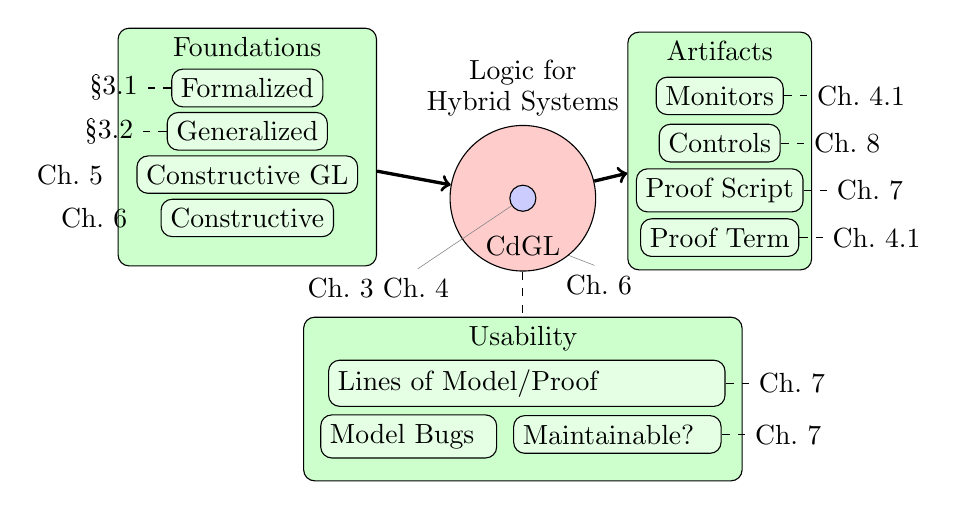
\begin{tikzpicture}[scale=0.5]
\draw (0,3.2)  node {Logic for};
\draw (0,2.4)  node {Hybrid Systems};
\draw (0,0)   node[circle]      (CdGLcirc) {\phantom{\hspace{1.1cm}}};
\draw (0,-1) node (cdgl) {\phantom{\CdGL}};
\node[coordinate,pin={[pin distance=0.55cm,text width=2cm]320:{Ch.\ 6}}] (cdgl-ref) at (cdgl) {};
\draw (0,0)   node[circle, fill=red!20,draw]      (CdGLcirc) {\phantom{\hspace{1.6cm}}};
\draw (0,-1.2) node (cdgl) {\CdGL};
\draw (0,0)   node[circle]  (dl)  {\phantom{\dL}};
\node[coordinate,pin={[pin distance=0.9cm,text width=3cm]265:{\ \ \ \ Ch.\ 3 Ch.\ 4}}] (dl-ref) at (dl) {};
\draw (dl) node[circle, fill=blue!20,draw]  {\dL};
\draw (-7, 1.3) node[rectangle,rounded corners,fill=green!20,draw,text depth=1in,text width=1.2in,text centered] (logic) {Foundations};
\draw (-7, 2.8) node[rectangle,rounded corners,fill=green!10,draw,thin,minimum height=0.3cm] (formalization) {\dL Formalized};
\draw (-7, 1.7) node[rectangle,rounded corners,fill=green!10,draw,thin,minimum height=0.3cm] (generalization) {\dL Generalized};
\draw (-7, 0.6) node[rectangle,rounded corners,fill=green!10,draw,thin,minimum height=0.3cm] (cgl) {Constructive \GL};
\draw (-7, -0.5) node[rectangle,rounded corners,fill=green!10,draw,thin,minimum height=0.3cm] (cdgl) {Constructive \dGL};
\draw node[left=0.3cm of formalization] (formal-ref) {\S3.1};
\draw node[left=0.3cm of generalization] (gen-ref) {\S3.2};
\draw node[left=0.3cm of cgl] (cgl-ref) {Ch.\ 5};
\draw node[left=0.3cm of cdgl] (cdgl-ref) {Ch.\ 6};
\draw[dashed] (formalization) -- (formal-ref);
\draw[dashed] (generalization) -- (gen-ref);
\draw (5, 1.2) node[rectangle,rounded corners,fill=green!20,draw,text depth=1in,text width=2.1cm,text centered] (engine) {Artifacts};
\draw (5, 2.6) node[rectangle,rounded corners,fill=green!10,draw,thin,minimum height=0.3cm] (monitors) {Monitors};
\draw (5, 1.4) node[rectangle,rounded corners,fill=green!10,draw,thin,minimum height=0.3cm] (controllers) {Controls};
\draw (5, 0.2) node[rectangle,rounded corners,fill=green!10,draw,thin,minimum height=0.3cm] (proofscript) {Proof Script};
\draw (5, -1) node[rectangle,rounded corners,fill=green!10,draw,thin,minimum height=0.3cm] (proofterm) {Proof Term};
\draw node[right=0.3cm of monitors] (monitor-ref) {Ch.\ 4.1};
\draw node[right=0.3cm of controllers] (controllers-ref) {Ch.\ 8};
\draw node[right=0.3cm of proofscript] (proofscript-ref) {Ch.\ 7};
\draw node[right=0.3cm of proofterm] (proofterm-ref) {Ch.\ 4.1};
\draw[dashed] (monitors) -- (monitor-ref);
\draw[dashed] (controllers) -- (controllers-ref);
\draw[dashed] (proofscript) -- (proofscript-ref);
\draw[dashed] (proofterm) -- (proofterm-ref);
\node[shape=coordinate] (use-anchor) at (0,-3){};
%\draw (1.45,-2) -- (0,-2.7);
\draw (0, -5.1) node[rectangle,rounded corners,fill=green!20,draw,text depth=1.6cm,text width=2.1in,text centered] (luser) {Usability};
%\draw (0, -3.1) node[rectangle,rounded corners,fill=green!10,draw,thin,minimum height=0.3cm] (monitors)    {Simplicity};
\draw (0.3, -4.7) node[rectangle,rounded corners,fill=green!10,draw,thin,minimum height=0.3cm] (monitors)    {Simplicity};
\draw (0.1, -4.7) node[rectangle,rounded corners,fill=green!10,draw,thin,minimum height=0.3cm,text width=4.8cm] (lop)    {Lines of Model/Proof};
%\draw (0, -4.15) node[rectangle,rounded corners,fill=green!10,draw,thin,minimum height=0.3in,text width=0.7in] (controllers) {Modeling Mistakes};
\draw (-2.9, -6.05) node[rectangle,rounded corners,fill=green!10,draw,thin,minimum height=0.3cm,text width=2cm] (modelmistake) {Model Bugs};
\draw (2.4, -6) node[rectangle,rounded corners,fill=green!10,draw,thin,minimum height=0.3cm,text width=2.4cm] (maintainable) {Maintainable?};
\draw node[right=0.3cm of maintainable] (maintain-ref) {Ch.\ 7};
\draw node[right=0.3cm of lop] (lop-ref) {Ch.\ 7};
\draw[->,very thick] (logic) -- (CdGLcirc);
\draw[->,very thick] (CdGLcirc) -- (engine);
\draw[dashed] (CdGLcirc) -- (luser);
\draw[dashed] (lop) -- (lop-ref);
\draw[dashed] (maintainable) -- (maintain-ref);
\end{tikzpicture}
\end{center}
%  \caption{Goals of the thesis}
%  \label{fig:goals-diagram}
%\end{figure}
\end{frame}

\begin{frame}[t]{Thesis is Big, but Doable}
Timeline: $\approx$\textbf{1 year}, optimistic
\begin{itemize}
\item 3 months (Sep-Nov) Extend \CGL theory to \CdGL theory (Submit to IJCAR around February 2020)
\item 3 months (Dec-Feb) Implement Kaisar with \CdGL proof checking (Submit to ITP or FM late March 2020)
\item 2 months: (Mar-Apr) Develop \ProofPlex implementation (Submit to  RV, May 2020, or if finished early, CAV in February 2020)
\item 1 month: (May) Generalize ground robotics case study to \CdGL
\item 3 months: (June-August) Write thesis document, defend
\end{itemize}
Kaisar builds on prior prototype, \CdGL builds on existing \CGL $\rightsquigarrow$ less ``rampup'' needed
\end{frame}

\begin{frame}[t,allowframebreaks]{Backup Plans are in Place}
\textbf{CdGL Backup Plans:}
\begin{itemize}
\item If $\ddiamond{\text{ODE}}{}$ rules are infeasible, pursue simplified ``solve'' axiom
\item If arbitrary computable terms are infeasible, use polynomial terms with limited use of semialgebraic witnesses
\item If model-predictive control is infeasible, focus on synthesizing assignments and conditionals
\item If refinement work fails, can directly reimplement sandboxing on games or rely on manual refinement
\end{itemize}

\textbf{Kaisar Backup Plans:}
\begin{itemize}
\item If usability results are weak, extend theory results
\item If nominal features do not provide desired benefits, refocus efforts on modularity
\item If implementation tasks become infeasibly large, pursue tighter integration with \KeYmaeraX code base or cut ``Export to Bellerophon proof'' feature
\end{itemize}

{\textbf{Robot Backup Plans:}
\begin{itemize}
\item Pursue a mix of hardware and simulation evaluations based on needs
\item Generalize robot model to improve synthesized monitor
\item Minimize proof complexity to support easy synthesis
\end{itemize}}
\end{frame}


\begin{frame}[t]{Thesis Makes the Whole Crew Happy}
  \begin{tabular}{lll}
    \ah{1}{\engineer} & \ah{1}{\logician} & \ah{1}{\logicuser}\\
    \acl{1}{\sayHappy{Full synthesis suite!}} & \acl{1}{\sayHappy{Formal foundations!}} & \acl{1}{\sayHappy{Structured proofs!}}
  \end{tabular}
\end{frame}

\begin{frame}[t,allowframebreaks]{TODO List}
  \begin{itemize}
  \item Monday: Develop figures for last section
  \item Time the talk
  \item Identify nonsense slides, e.g., where background info, connecting info, explanation, context are needed.
  \item Try to fix nonsense by Tuesday meeting. 
  \item In meeting, discuss: Slides, resubmission plans, whether to do extra practice talks


  \item Research related works which inform design questions, e.g., Isar architecture and software engineering works
  \item Identify questions likely to be asked by committee, prepare answers
  \item Identify additional figures that improve slides, make said figures
  \item General polish
  \item Practice talk in lab meeting, Oct 22
  \item Test Skype connection with Tobias
  \item Keep document updated with insights and plans arising from the talk editing, and publishing status
  \end{itemize}
\end{frame}

\appendix
\section<presentation>*{\appendixname}
\subsection<presentation>*{For Further Reading}

\begin{frame}[t, allowframebreaks]
\frametitle{References}
\bibliographystyle{amsalpha}
\bibliography{proposal,platzer,verified-pipeline,hilbert-epsilons,ground-robotics,verified-dL,constructive-games,kaisar}
\end{frame}

\end{document}